\documentclass[12pt,a4paper]{ctexart}

\usepackage{../../Styles/mystyle-report}

\graphicspath{{./image/}}% 指定图片目录，后续可以直接使用图片文件名。

% 图表标题格式
\renewcommand{\figurename}{图}
\renewcommand{\tablename}{表}

\geometry{left=2.5cm,right=2.5cm,top=2.5cm,bottom=2.5cm} % 页边距

% 超链接设置
\hypersetup{
colorlinks=true, linkcolor=black, citecolor=black, urlcolor=blue
}

\pagestyle{fancy}
\fancyhf{} % 清空默认页眉页脚

% 页眉：右侧章节，左侧页码（右侧页码去掉了)
% \fancyhead[L]{\zihao{5} \thepage}
\fancyhead[R]{\zihao{5} \leftmark}

% 页码放到 页面底部 正中间
\fancyfoot[C]{\zihao{5} \thepage}

% 页眉细横线
\renewcommand{\headrulewidth}{0.5pt}

% 让\section自动生成页眉标记
\renewcommand{\sectionmark}[1]{\markboth{\thesection\quad #1}{}}

% 核心：开启4级标题编号 + 定义四级标题
\setcounter{secnumdepth}{4}% 让四级标题显示编号
\setcounter{tocdepth}{4}% 让四级标题出现在目录
\let\subsubsubsection\paragraph% 定义命令：\subsubsubsection 等价于四级标题




\begin{document}

% 标题
\title{\heiti 基于ARMA-EGARCH模型的国际原油价格时间序列分析}
\author{邹文杰}
\date{\today}
\maketitle

% 摘要
\begin{abstract}

\noindent\textbf{关键词：}
\end{abstract}

\newpage
\tableofcontents% 添加目录
\markboth{目录}{目录} % 目录页页眉显示“目录”

\newpage
\section{引言}

国际原油价格波动深刻影响着全球经济运行、能源安全及金融市场稳定。WTI、Brent和Dubai三大基准原油分别代表北美、欧洲和亚太三大区域市场，其价格波动特征既存在共性，又因市场结构差异而呈现不同特征。准确刻画原油价格的波动规律对投资决策、风险管理及政策制定具有重要意义。

传统时间序列模型通常假设扰动项同方差，但金融资产收益率序列普遍存在波动聚集和杠杆效应。自Engle(1982)提出ARCH模型以来，GARCH族模型成为刻画金融波动的主流工具。其中，EGARCH模型能够捕捉波动非对称性，且无需对参数施加非负约束，更适用于原油等大宗商品市场。

本文选取1992年1月至2026年3月WTI、Brent和Dubai原油月度价格数据，首先对对数收益率序列构建ARMA均值模型，然后基于t分布构建EGARCH族模型，系统对比三大原油的波动特征，为市场参与者提供量化参考。

\section{数据来源与预处理}
\subsection{数据基本信息介绍}

本文选取全球三大原油基准价格作为研究对象，分别为：西德克萨斯中质原油（WTI）、布伦特原油（Brent）及迪拜原油（Dubai），其基本信息如下：
\begin{itemize}
\item 数据名称：

Global price of WTI Crude (POILWTIUSDM)，

Global price of Brent Crude (POILBREUSDM)，

Global price of Dubai Crude (POILDUBUSDM)，

\item 数据来源：

\url{https://fred.stlouisfed.org/series/POILWTIUSDM}，

\url{https://fred.stlouisfed.org/series/POILBREUSDM}，

\url{https://fred.stlouisfed.org/series/POILDUBUSDM}，

\item 数据频率：月度数据；时间跨度：1992年1月—2026年3月

\item 分析软件：EViews 13

\item 三大原油价格的基各项指标如表~\ref{tab:crude_oil_benchmark}所示。
\begin{table}[H]
\centering
\caption{三大原油基准价格各项指标说明}
\label{tab:crude_oil_benchmark}
% 自适应文本宽度，自动换行
\begin{tabularx}{\textwidth}{l l X c c X}
\toprule
$\,\,\,\,\,\,\,\,$系列代号 & 名称 & $\quad\,\,\,\,$本质 & 产地 & 品质 & $\,\,\,$定价基准 \\
\midrule
POILWTIUSDM   & WTI     & 西德克萨斯中质原油 & 美国得州 & 轻质低硫 & 北美原油贸易基准 \\
POILBREUSDM   & Brent   & 北海布伦特原油     & 欧洲北海 & 轻质低硫 & 全球原油贸易核心基准 \\
POILDUBUSDM   & Dubai   & 迪拜原油           & 中东阿联酋 & 中质含硫 & 亚太原油进口基准 \\
\bottomrule
\end{tabularx}
\end{table}
\end{itemize}


\subsection{数据预处理}
为消除量纲影响和平滑波动，分别对原始序列POILWTIUSDM、POILBREUSDM、POILDUBUSDM做对数变换得
\begin{align}
&\mathrm{LN}\_\mathrm{WTI}=\ln \left( \mathrm{POILWTIUSDM} \right) ,
\\
&\mathrm{LN}\_\mathrm{BRENT}=\ln \left( \mathrm{POILBREUSDM} \right) ,
\\
&\mathrm{LN}\_\mathrm{DUBAI}=\ln \left( \mathrm{POILDUBUSDM} \right) ,
\end{align}
其时序图如图~\ref{fig:对数序列时序图}所示。
\begin{figure}[H]
\centering
% 第一行：2张图（WTI + BRENT）
\begin{minipage}{0.48\textwidth}
\centering
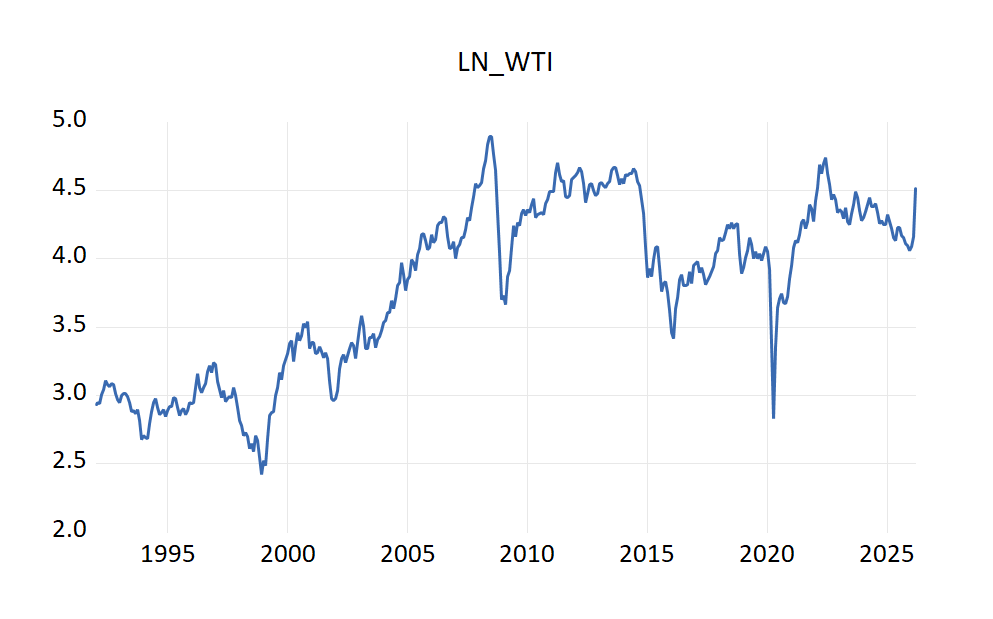
\includegraphics[width=\linewidth]{序列ln_wti时序图.png}
\end{minipage}
\hfill
\begin{minipage}{0.48\textwidth}
\centering
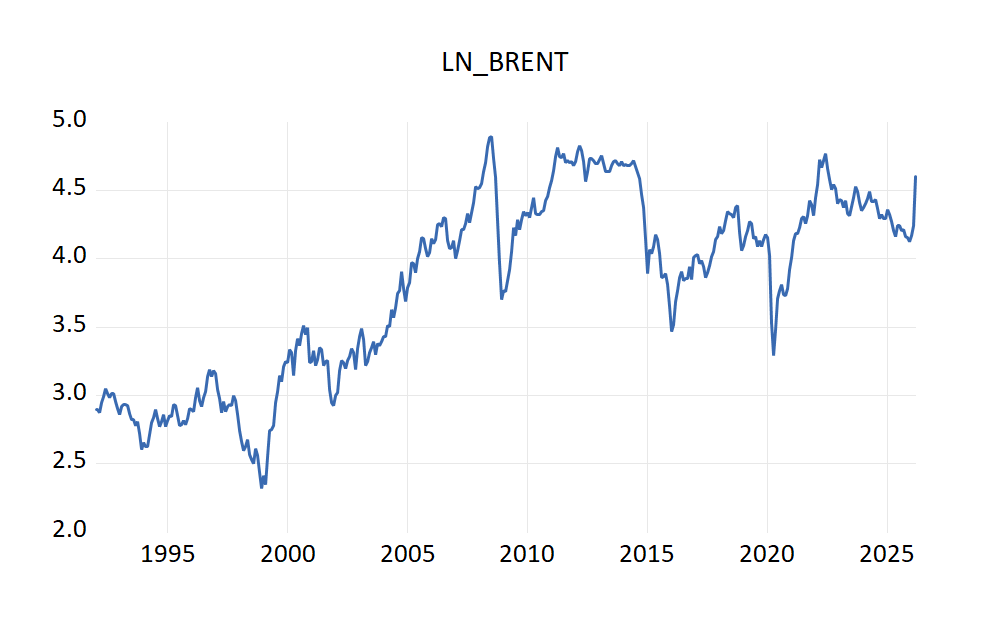
\includegraphics[width=\linewidth]{序列LN_BRENT时序图.png}
\end{minipage}

\vspace{1em} % 上下行间距
% 第二行：1张图居中（Dubai）
\begin{minipage}{0.48\textwidth}
\centering
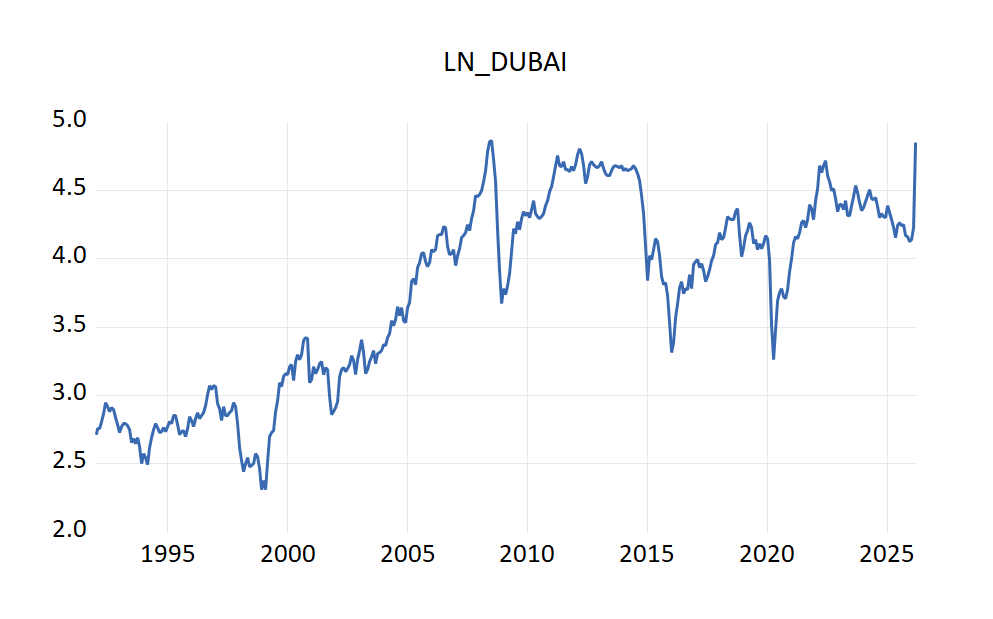
\includegraphics[width=\linewidth]{序列ln_dubai时序图.png}
\end{minipage}

\caption{三大原油价格对数序列时序图}
\label{fig:对数序列时序图}
\end{figure}

\section{构建序列LN\_WTI的时间序列模型}

\subsection{平稳性与非白噪声检验}

\subsubsection{ADF单位根检验}

对序列LN\_WTI做三种情形的ADF单位根检验，结果如图~\ref{fig:序列LN_WTI的ADF检验结果图}所示。
\begin{figure}[H]
\centering
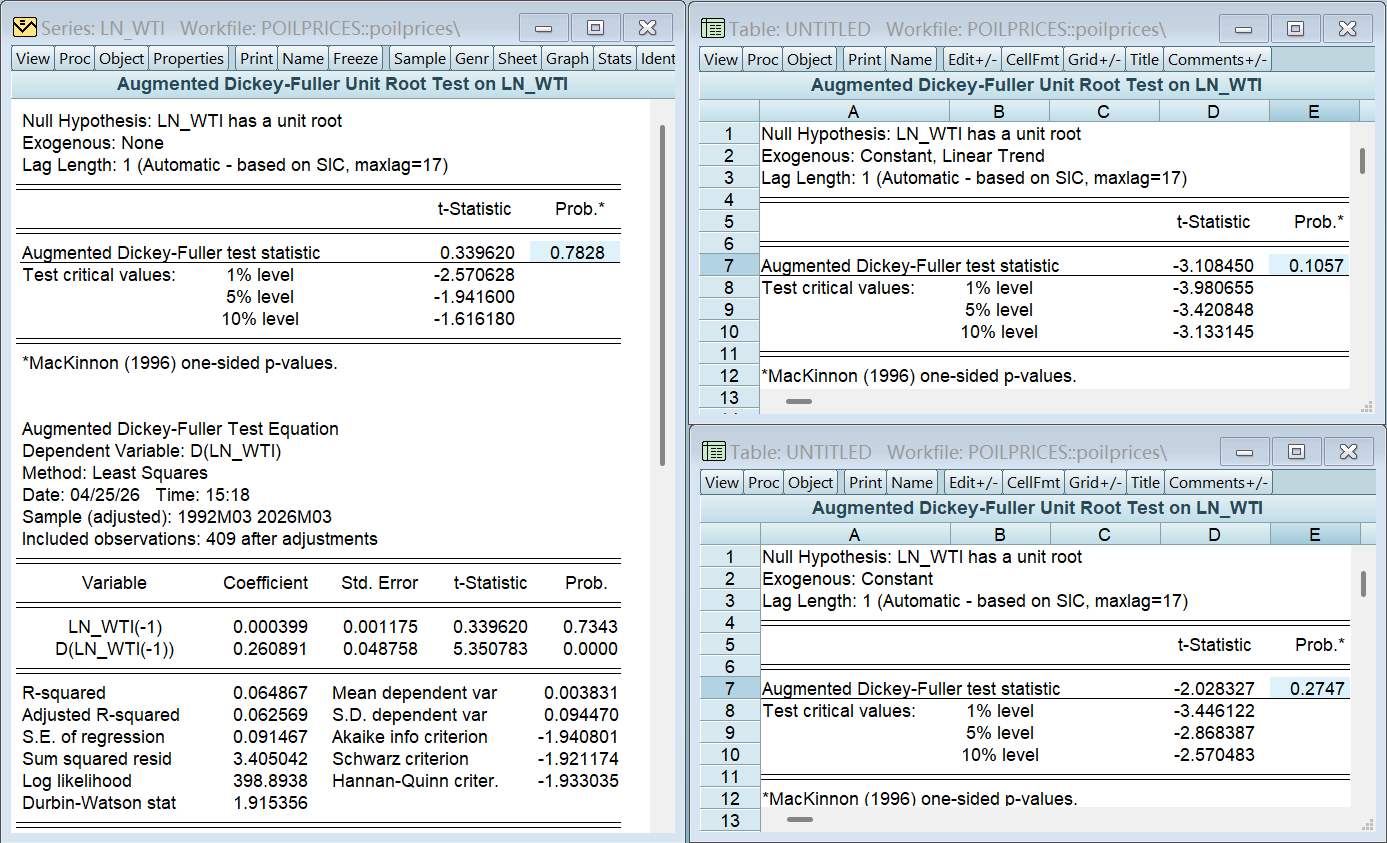
\includegraphics[width=0.8\textwidth]{序列LN_WTI的ADF检验结果图.png}
\caption{序列LN\_WTI的ADF检验结果图}
\label{fig:序列LN_WTI的ADF检验结果图}
\end{figure}
由图~\ref{fig:序列LN_WTI的ADF检验结果图}可知，序列LN\_WTI三种情形的P值均大于0.05，在5\%显著水平下均无法拒绝 “序列存在单位根” 的原假设。这说明，序列LN\_WTI在三种检验设定下均存在单位根、不满足平稳性要求。因此，后续建模不能直接对原序列建立 ARMA 模型，需要先对序列进行差分处理，再对差分后的序列重新进行单位根检验，根据差分后的平稳性结果选择对应的模型形式。

对序列LN\_WTI做一阶差分得序列
\begin{align}
\mathrm{DF}\_\mathrm{LN}\_\mathrm{WTI}=\mathrm{LN}\_\mathrm{WTI}_t-\mathrm{LN}\_\mathrm{WTI}_{t-1},
\end{align}
其时序图如图~\ref{fig:序列DF_LN_WTI时序图}所示。
\begin{figure}[H]
\centering
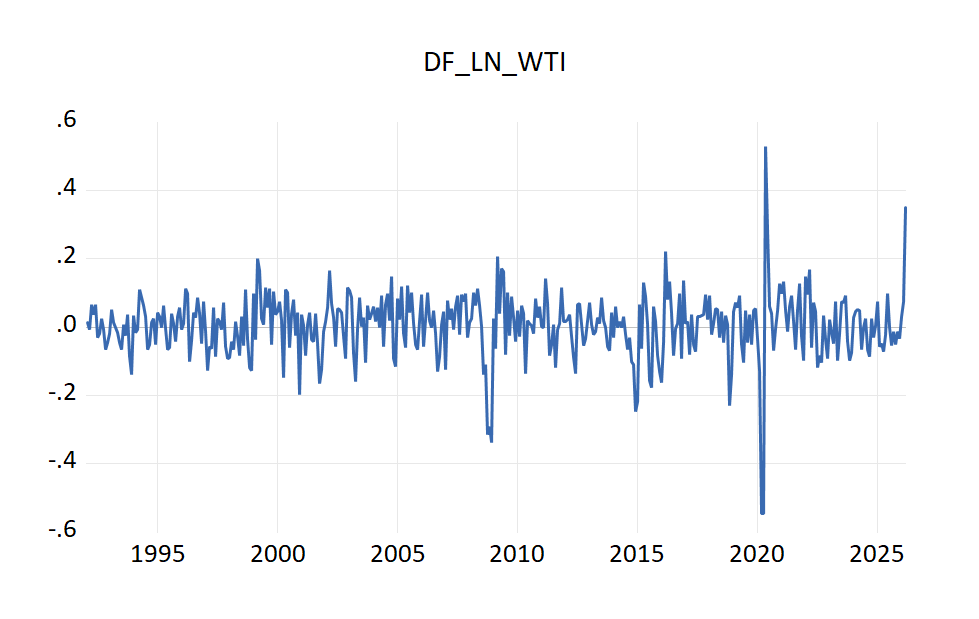
\includegraphics[width=0.8\textwidth]{序列df_ln_wti时序图.png}
\caption{序列DF\_LN\_WTI时序图}
\label{fig:序列DF_LN_WTI时序图}
\end{figure}

再对序列DF\_LN\_WTI做三种情形的ADF单位根检验，结果如图~\ref{fig:序列DF_LN_WTI的ADF检验结果图}所示。
\begin{figure}[H]
\centering
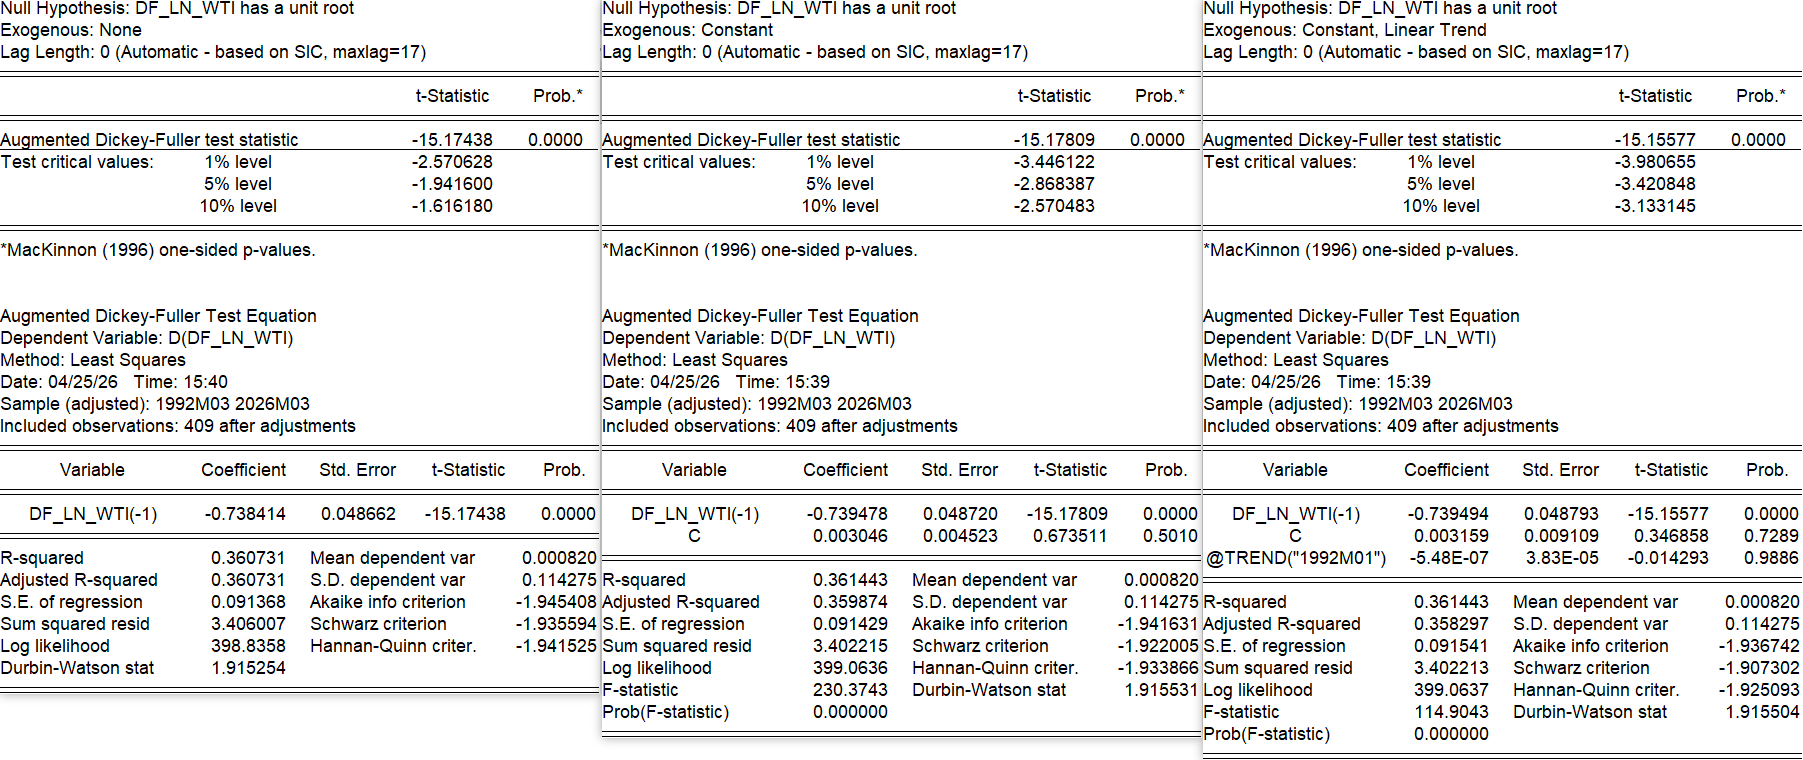
\includegraphics[width=0.8\textwidth]{序列DF_LN_WTI的ADF检验结果图.png}
\caption{序列DF\_LN\_WTI的ADF检验结果图}
\label{fig:序列DF_LN_WTI的ADF检验结果图}
\end{figure}

由图~\ref{fig:序列DF_LN_WTI的ADF检验结果图}可知，序列DF\_LN\_WTI三种情形的p值均小于0.05，在5\%显著性水平下均拒绝 “序列存在单位根” 的原假设。这说明，序列DF\_LN\_WTI在三种检验设定下均不存在单位根、满足平稳性要求。再将图~\ref{fig:序列DF_LN_WTI的ADF检验结果图}中三种情形的AIC/SC/HQ值汇总到表~\ref{table:序列DF_LN_WTI单位根检验不同情形的信息准则对比}中。
\begin{table}[H]
\centering
\caption{序列DF\_LN\_WTI单位根检验不同情形的信息准则对比}
\label{table:序列DF_LN_WTI单位根检验不同情形的信息准则对比}
\begin{tabular}{lccc}
\toprule[1.2pt] % 顶部粗线
检验设定 & AIC准则 & SC准则 & HQ准则 \\
\midrule[0.75pt] % 中间细线
None & $\mathbf{-1.945408}$ & $\mathbf{-1.935594}$& $\mathbf{-1.941525}$ \\
Constant & -1.941631 & -1.922005 & -1.933866 \\
Constant,Linear Trend & -1.936742 & -1.907302 & -1.925093 \\
\bottomrule[1.2pt] % 底部粗线
\end{tabular}
\end{table}

根据AIC/SC/HQ准则，最终选择\textbf{无截距项、无时间趋势}$(\mathbf{None})$的情形，故可对序列DF\_LN\_WTI构建\textbf{无截距、无时间趋势的}$\mathbf{ARMA}$\textbf{模型}。


\subsubsection{自相关与偏自相关函数分析}

序列DF\_LN\_WTI的自相关与偏自相关函数检验结果如图~\ref{fig:序列DF_LN_WTI的ACF和PACF相关图}所示。
\begin{figure}[H]
\centering
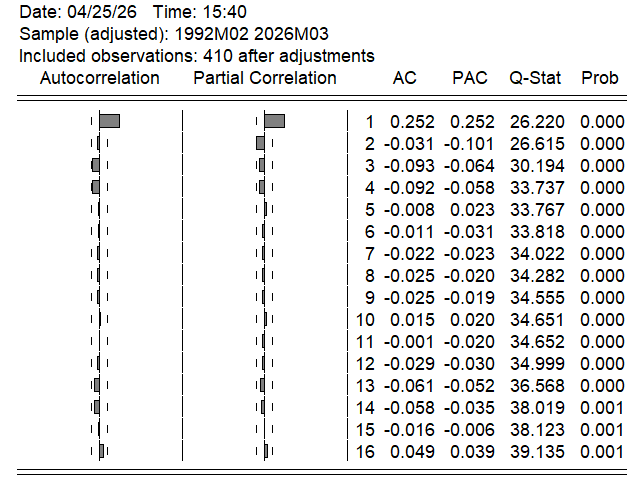
\includegraphics[width=0.8\textwidth]{序列DF_LN_WTI的ACF和PACF相关图.png}
\caption{序列DF\_LN\_WTI的ACF和PACF相关图}
\label{fig:序列DF_LN_WTI的ACF和PACF相关图}
\end{figure}

由图~\ref{fig:序列DF_LN_WTI的ACF和PACF相关图}可知
\begin{itemize}
\item 滞后 1 至 16 阶的 Q 统计量伴随概率（p 值）均小于 0.05 的显著性水平，因此拒绝 “序列为白噪声” 的原假设，表明序列DF\_LN\_WTI存在显著的自相关性，并非独立同分布的白噪声序列，具备构建时间序列模型的基础。

\item 自相关函数（ACF）仅滞后 1 阶系数显著不为 0，滞后 2 阶及以后的系数绝对值均小于临界值，呈现\textbf{1阶截尾}特征；偏自相关函数（PACF）在滞后 1 阶、滞后 2 阶显著不为 0，自滞后 3 阶起所有系数均未通过显著性检验，呈现\textbf{2阶截尾}特征。
\end{itemize}


\subsection{ARMA模型构建与检验}


\subsubsection{模型构建与优选}

根据之前对序列DF\_LN\_WTI的自相关函数（ACF）和偏自相关函数（PACF）的特征分析，构建AR(1)、AR(2)、MA(1)、MA(2)、ARMA(1,1)、ARMA(1,2)、ARMA(2,1)、ARMA(2,2)模型，再残差检验和信息准则筛选最优模型。各个模型的结果如图~\ref{fig:序列DF_LN_WTI的AR、MA模型结果图}和图~\ref{fig:序列DF_LN_WTI的ARMA模型结果图}所示。
\begin{figure}[H]
\centering
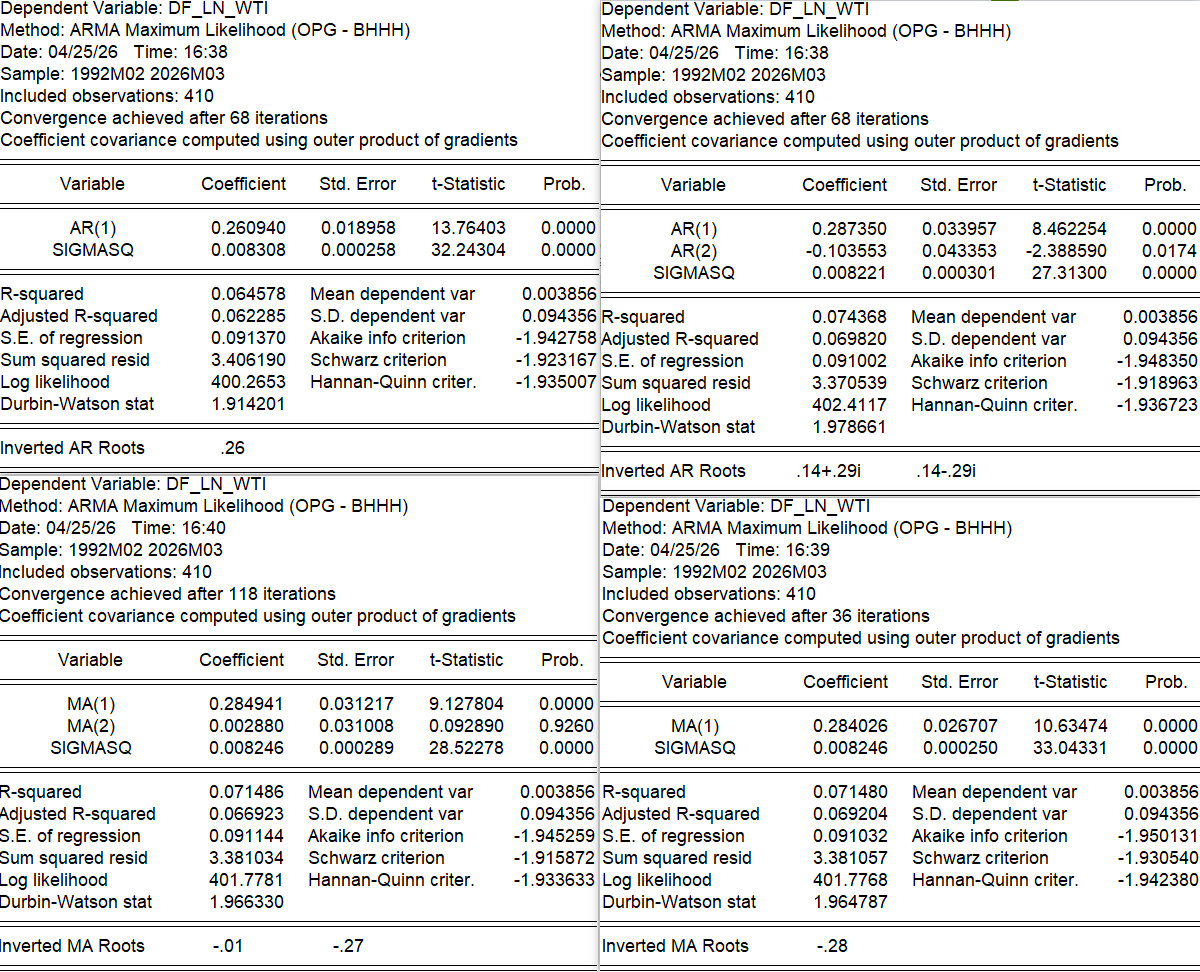
\includegraphics[width=0.8\textwidth]{序列DF_LN_WTI的AR、MA模型结果图.png}
\caption{序列DF\_LN\_WTI的AR、MA模型结果图}
\label{fig:序列DF_LN_WTI的AR、MA模型结果图}
\end{figure}

\begin{figure}[H]
\centering
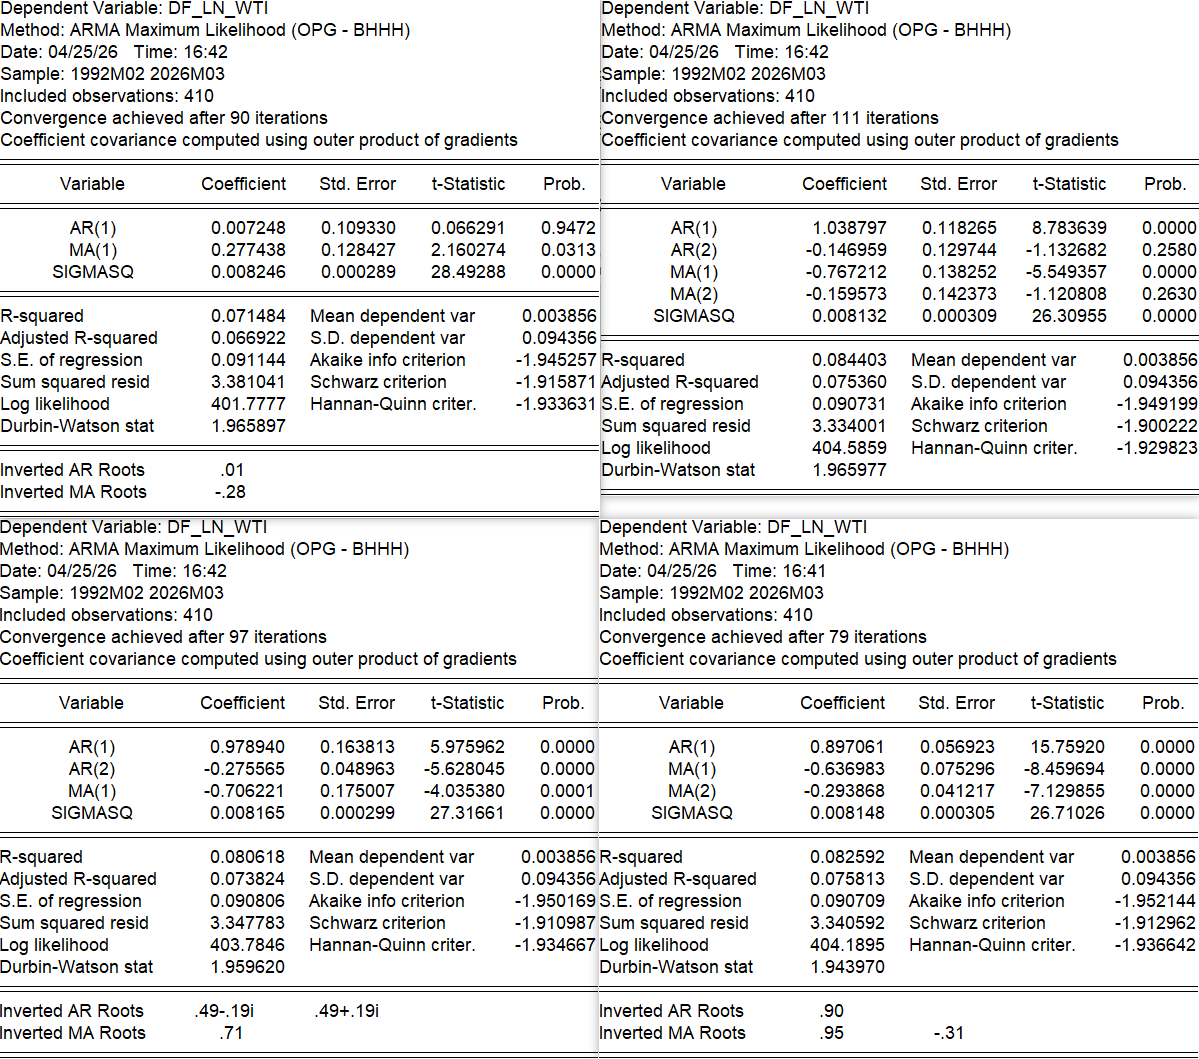
\includegraphics[width=0.8\textwidth]{序列DF_LN_WTI的ARMA模型结果图.png}
\caption{序列DF\_LN\_WTI的ARMA模型结果图}
\label{fig:序列DF_LN_WTI的ARMA模型结果图}
\end{figure}

将图~\ref{fig:序列DF_LN_WTI的AR、MA模型结果图}和图~\ref{fig:序列DF_LN_WTI的ARMA模型结果图}中各个模型的系数显著性检验结果和AIC/SC/HQ值分别汇总到如下表~\ref{tab:arma_pvalue_new}和表~\ref{tab:arma_criteria_new}中。
\begin{table}[H]
\centering
\caption{ARMA模型系数显著性检验结果}
\label{tab:arma_pvalue_new}
\begin{tabular}{cccccc}
\toprule[1.2pt]
模型  & AR(1) & AR(2) & MA(1) & MA(2) \\
\midrule[0.75pt]
ARMA(1,1)  & 0.9472 & - & 0.0313 & - \\
ARMA(2,2)  & 0.0000 & 0.2580 & 0.0000 & 0.2630 \\
ARMA(2,1)  & 0.0000 & 0.0000 & 0.0001 & - \\
ARMA(1,2)  & 0.0000 & - & 0.0000 & 0.0000 \\
AR(1)      & 0.0000 & - & - & - \\
AR(2)      & 0.0000 & 0.0174 & - & - \\
MA(1)      & - & - & 0.0000 & - \\
MA(2)      & - & - & 0.0000 & 0.9260 \\
\bottomrule[1.2pt]
\end{tabular}
\end{table}

\begin{table}[H]
\centering
\caption{ARMA模型信息准则对比结果}
\label{tab:arma_criteria_new}
\begin{tabular}{cccc}
\toprule[1.2pt]
模型 & AIC & SC & HQ \\
\midrule[0.75pt]
ARMA(1,1) & -1.9453 & -1.9159 & -1.9336 \\
ARMA(2,2) & -1.9492 & -1.9002 & -1.9298 \\
ARMA(2,1) & -1.9502 & -1.9109 & -1.9347 \\
ARMA(1,2) & -1.9521 & -1.9130 & -1.9366 \\
AR(1)     & -1.9428 & -1.9232 & -1.9350 \\
AR(2)     & -1.9483 & -1.9189 & -1.9367 \\
MA(1)     & $\mathbf{-1.9501}$ & $\mathbf{-1.9305}$ & $\mathbf{-1.9424}$ \\
MA(2)     & -1.9453 & -1.9159 & -1.9336 \\
\bottomrule[1.2pt]
\end{tabular}
\end{table}
根据系数显著性和AIC/SC/HQ信息准则，再结合表~\ref{tab:arma_pvalue_new}和表~\ref{tab:arma_criteria_new}，最终选择 $\mathbf{MA}(\mathbf{1})$\textbf{模型}进行后续建模与分析。其余模型或存在参数不显著的问题，或在信息准则上表现略逊，因此不予采用。

\subsubsection{适应性检验}

对序列DF\_LN\_WTI的MA(1)模型的残差序列做Q检验，结果如图~\ref{fig:序列DF_LN_WTI的MA(1)模型的适应性检验结果图}所示。
\begin{figure}[H]
\centering
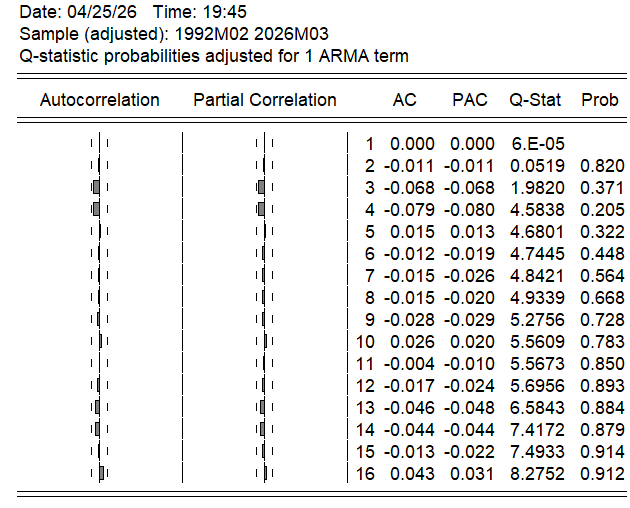
\includegraphics[width=0.8\textwidth]{序列DF_LN_WTI的MA(1)模型的适应性检验结果图.png}
\caption{序列DF\_LN\_WTI的MA(1)模型的适应性检验结果图}
\label{fig:序列DF_LN_WTI的MA(1)模型的适应性检验结果图}
\end{figure}

由图~\ref{fig:序列DF_LN_WTI的MA(1)模型的适应性检验结果图}可知
\begin{itemize}
\item 滞后2至16阶的Q统计量伴随概率均大于0.05的显著性水平，无法拒绝“残差序列为白噪声”的原假设。

\item 残差序列的自相关函数（ACF）与偏自相关函数（PACF）在各滞后阶数的系数绝对值均未超出95\%置信区间，无显著自相关性，表明MA(1)模型已充分提取原序列的均值自相关信息。
\end{itemize}

\subsubsection{条件异方差检验}

考虑到条件异方差多表现为短期波动聚集，低阶滞后项已能捕捉绝大多数 ARCH 效应；同时，滞后阶数过高会导致检验自由度下降、估计偏差增大，故本文只选取滞后 4、5、6 阶进行 ARCH-LM 检验。现在对序列DF\_LN\_WTI的MA(1)模型的残差分别做滞后4、5、6阶的ARCH效应检验，结果如图~\ref{fig:序列DF_LN_WTI的MA(1)模型的ARCH效应检验}所示。
\begin{figure}[H]
\centering
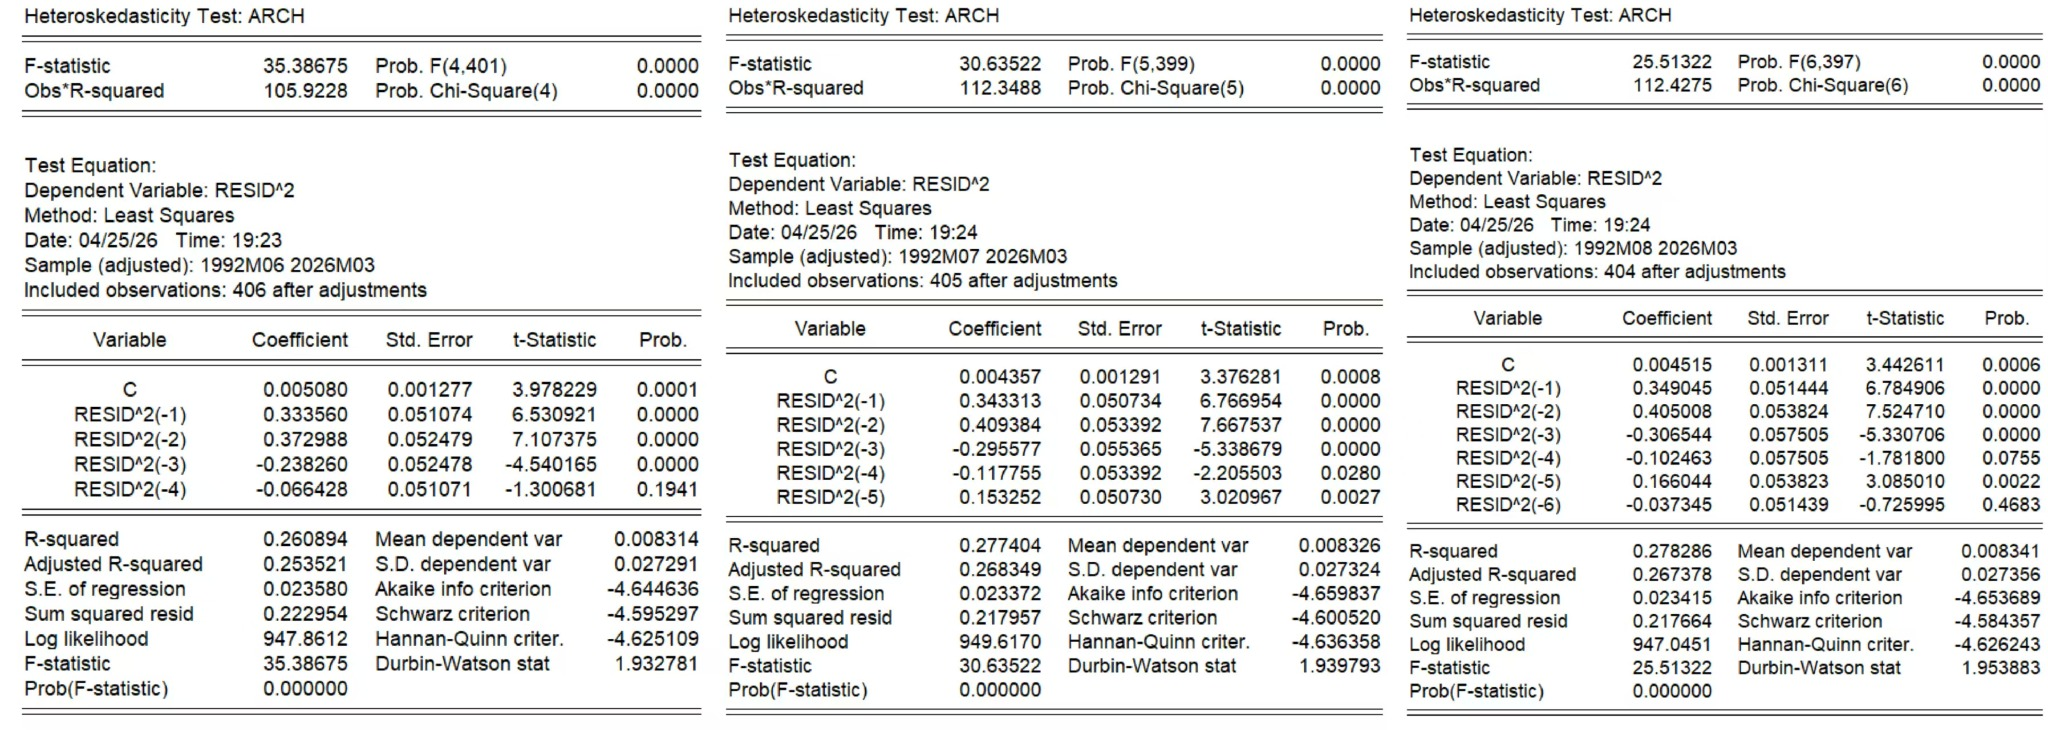
\includegraphics[width=0.8\textwidth]{序列DF_LN_WTI的MA(1)模型的ARCH效应检验.png}
\caption{MA(1)模型的ARCH效应检验}
\label{fig:序列DF_LN_WTI的MA(1)模型的ARCH效应检验}
\end{figure}

图~\ref{fig:序列DF_LN_WTI的MA(1)模型的ARCH效应检验}的结果显示：在三种滞后阶数下，F 统计量与 LM 统计量的 p 值均显著为 0.0000<0.05，表明残差平方序列存在显著的条件异方差性。

再对序列的残差平方做检验，结果如图~\ref{fig:序列DF_LN_WTI的MA(1)模型残差的平方的Q检验结果图}所示。
\begin{figure}[H]
\centering
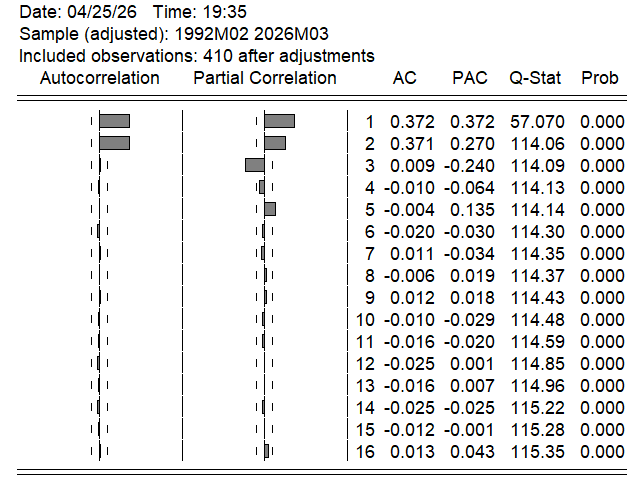
\includegraphics[width=0.8\textwidth]{序列DF_LN_WTI的MA(1)模型残差的平方的Q检验结果图.png}
\caption{MA(1)模型残差的平方的Q检验结果图}
\label{fig:序列DF_LN_WTI的MA(1)模型残差的平方的Q检验结果图}
\end{figure}

由图~\ref{fig:序列DF_LN_WTI的MA(1)模型残差的平方的Q检验结果图}可知
\begin{itemize}
\item 滞后1至16阶的Q统计量的伴随概率均小于0.01，在1\%的显著性水平下强烈拒绝“残差平方序列不存在自相关”的原假设。

\item 残差平方序列的自相关函数（ACF）在滞后1阶（系数为0.372）、滞后2阶（系数为0.371）均显著不为0，呈现出明显的自相关性，表明残差序列存在显著的波动率聚集性特征。
\end{itemize}

上述两种检验的结果说明，序列DF\_LN\_WTI的MA(1)模型的残差序列存在显著的条件异方差，不满足经典时间序列模型的同方差假设。为此，本文进一步构建 GARCH 类模型，以同时刻画序列的均值过程与异方差特征。


\subsection{GARCH族模型构建与检验}

序列DF\_LN\_WTI的直方图与描述性统计如图~\ref{fig:序列DF_LN_WTI的直方图与描述性统计图}所示。
\begin{figure}[H]
\centering
\includegraphics[width=0.8\textwidth]{序列DF_LN_WTI的直方图与描述性统计图.png}
\caption{序列DF\_LN\_WTI的直方图与描述性统计图}
\label{fig:序列DF_LN_WTI的直方图与描述性统计图}
\end{figure}

由图~\ref{fig:序列DF_LN_WTI的直方图与描述性统计图}可知，序列DF\_LN\_WTI的峰度为10.85，显著大于正态分布的峰度3，且Jarque-Bera正态性检验的伴随概率为0.0000，强烈拒绝序列服从正态分布的原假设，表明该序列具有典型的\textbf{尖峰厚尾}特征。
传统GARCH模型的正态分布假设难以刻画金融时间序列的厚尾性，而t分布能够更好地拟合极端波动的尾部风险。基于此，本文后续构建的GARCH模型采用$\mathbf{t}$\textbf{分布}设定扰动项分布，以提升模型对序列波动特征的拟合效果。


\subsubsection{模型构建与优选}

基于序列DF\_LN\_WTI的尖峰厚尾特征与显著的条件异方差效应，对序列构建GARCH族模型，以估计序列的波动特征。

由于金融时间序列的异方差与波动持续性主要体现于短期滞后项，低阶GARCH模型即可有效刻画序列波动特征。过高滞后阶数易造成待估参数增多、拟合过度、参数估计不稳定等问题。因此本文在MA(1)均值方程基础上，只选取MA(1)-GARCH、MA(1)-TARCH、MA(1)-EGARCH三类低阶模型，并采用Student's t分布以适配序列DF\_LN\_WTI尖峰厚尾的统计特征。将各GARCH族模型系数显著性检验和信息准则结果分别汇总到表~\ref{tab:garch_pvalue_wti}和表~\ref{tab:garch_info_criteria_wti}中。

\begin{table}[H]
\centering
\caption{DF\_LN\_WTI序列GARCH族模型系数显著性检验结果}
\label{tab:garch_pvalue_wti}
\setlength{\tabcolsep}{8pt}
\begin{tabular}{lccccc}
\toprule[1.2pt]
模型名称           & 常数项C & ARCH项 & 非对称项 & GARCH项 \\
\midrule[0.75pt]
MA(1)-GARCH(1,0)-t     & \textbf{0.0000} & \textbf{0.0033} & - & - \\
MA(1)-GARCH(2,0)-t     & 0.0000 & 0.0400/0.0504 & - & - \\
MA(1)-GARCH(1,1)-t     & \textbf{0.0292} & \textbf{0.0075} & - & \textbf{0.0002} \\
MA(1)-GARCH(1,2)-t     & 0.0514 & 0.0280 & - & 0.2649/0.9921 \\
MA(1)-GARCH(2,1)-t     & \textbf{0.0617} & \textbf{0.0046}/\textbf{0.0042} & - & \textbf{0.0000} \\
MA(1)-GARCH(2,2)-t     & 0.1663/0.0122 & 0.0116 & - & 0.0000/0.0211 \\
\midrule
MA(1)-TARCH(1,0)-t     & 0.0000 & 0.7631 & 0.0012 & - \\
MA(1)-TARCH(2,0)-t     & 0.0000 & 0.7519/0.1519 & 0.0017 & - \\
MA(1)-TARCH(1,1)-t     & 0.0000 & 0.8927 & 0.0014 & 0.7877 \\
MA(1)-TARCH(1,2)-t     & 0.0000 & 0.9659 & 0.0004 & 0.0935/0.0513 \\
MA(1)-TARCH(2,1)-t     & 0.0000 & 0.9134/0.1907 & 0.0012 & 0.5160 \\
MA(1)-TARCH(2,2)-t     & 0.0000 & 0.8634/0.3143 & 0.0011 & 0.3208/0.4738 \\
\midrule
MA(1)-EGARCH(1,0)-t    & 0.0000 & 0.0625 & 0.0016 & - \\
MA(1)-EGARCH(2,0)-t    & 0.0000 & 0.1981/0.0000 & 0.0020 & - \\
MA(1)-EGARCH(1,1)-t    & \textbf{0.0113} & \textbf{0.0158} & \textbf{0.0193} & \textbf{0.0000} \\
MA(1)-EGARCH(1,2)-t    & 0.0232 & 0.0381 & 0.0121 & 0.0293/0.0797 \\
MA(1)-EGARCH(2,1)-t    & 0.0001 & 0.1802/0.0042 & 0.0028 & 0.6293 \\
MA(1)-EGARCH(2,2)-t    & 0.0104 & 0.1807/0.0272 & 0.0037 & 0.4647/0.0447 \\
\bottomrule[1.2pt]
\end{tabular}
\end{table}

\begin{table}[H]
\centering
\caption{DF\_LN\_WTI序列GARCH族模型信息准则结果对比}
\label{tab:garch_info_criteria_wti}
\setlength{\tabcolsep}{12pt}
\begin{tabular}{lcccc}
\toprule
模型名称          & MA(1)  & AIC      & SC       & HQ       \\
\midrule
MA(1)-GARCH(1,0)-t     & 0.0030 & -2.1922  & -2.1531  & -2.1767  \\
MA(1)-GARCH(2,0)-t     & 0.0001 & -2.2011  & -2.1520  & -2.1817  \\
MA(1)-GARCH(1,1)-t     & 0.0008 & -2.2037  & -2.1547  & -2.1843  \\
MA(1)-GARCH(1,2)-t     & 0.0008 & -2.1988  & -2.1400  & -2.1755  \\
MA(1)-GARCH(2,1)-t     & 0.0016 & -2.2082  & -2.1495  & -2.1850  \\
MA(1)-GARCH(2,2)-t     & 0.0005 & -2.2140  & -2.1418  & -2.1832  \\
\midrule
MA(1)-TARCH(1,0)-t     & 0.0000 & -2.2342  & -2.1852  & -2.2148  \\
MA(1)-TARCH(2,0)-t     & 0.0000 & -2.2377  & -2.1789  & -2.2144 \\
MA(1)-TARCH(1,1)-t     & 0.0000 & -2.2296  & -2.1708 & -2.2063  \\
MA(1)-TARCH(1,2)-t     & 0.0000 & -2.2323  & -2.1637  & -2.2052  \\
MA(1)-TARCH(2,1)-t     & 0.0000 & -2.2357  & -2.1671  & -2.2086  \\
MA(1)-TARCH(2,2)-t     & 0.0000 & -2.2332  & -2.1548  & -2.2022  \\
\midrule
MA(1)-EGARCH(1,0)-t    & 0.0000 & -2.1906  & -2.1417  & -2.1713  \\
MA(1)-EGARCH(2,0)-t    & 0.0000 & -2.2231  & -2.1644  & -2.1999  \\
MA(1)-EGARCH(1,1)-t    & 0.0000 & \textbf{-2.2182} & \textbf{-2.1594} & \textbf{-2.1949} \\
MA(1)-EGARCH(1,2)-t    & 0.0000 & -2.2155  & -2.1469  & -2.1883  \\
MA(1)-EGARCH(2,1)-t    & 0.0000 & -2.2187  & -2.1501  & -2.1915  \\
MA(1)-EGARCH(2,2)-t    & 0.0000 & -2.2252  & -2.1468  & -2.1942  \\
\bottomrule
\end{tabular}
\end{table}

由表~\ref{tab:garch_pvalue_wti}和表~\ref{tab:garch_info_criteria_wti}，再结合显著性检验和信息准则可知，$\mathbf{MA}(\mathbf{1})-\mathbf{EGARCH}(\mathbf{1},\mathbf{1})-\mathbf{t}$\textbf{模型}不仅所有参数均通过显著性检验，有效刻画了序列的杠杆效应与波动持续性，且信息准则表现最优，是刻画序列DF\_LN\_WTI波动特征的最优模型，其结果如图~\ref{fig:egarch11}所示。
\begin{figure}[H]
\centering
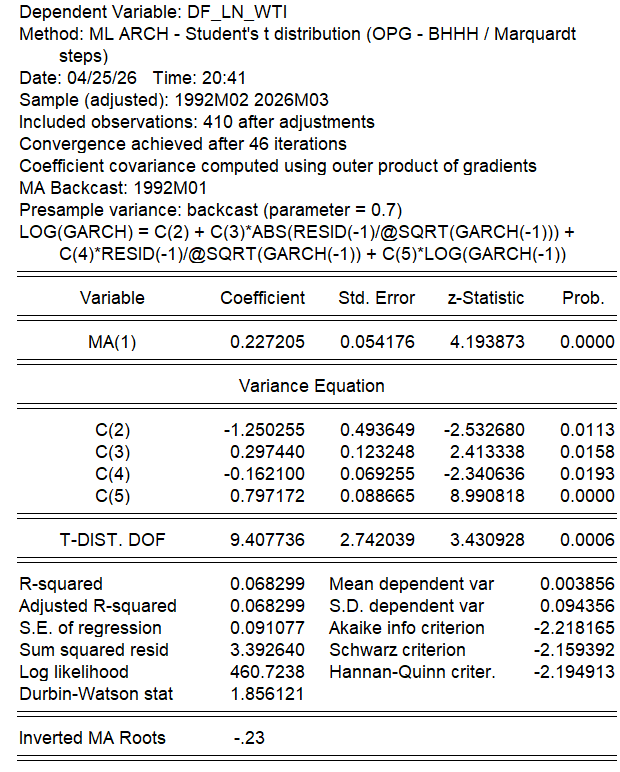
\includegraphics[width=0.7\textwidth]{序列LN_WTI的MA(1)-EGARCH(1,1)模型结果图.png}
\caption{MA(1)-EGARCH(1,1)-t模型估计结果图}
\label{fig:egarch11}
\end{figure}


\subsubsection{残差白噪声检验}

对序列DF\_LN\_WTI的MA(1)-EGARCH(1,1)-t模型的残差序列做Q检验，结果如图~\ref{fig:序列DF_LN_WTI的MA(1)-EGARCH(1,1)模型残差的Q检验结果图}所示。
\begin{figure}[H]
\centering
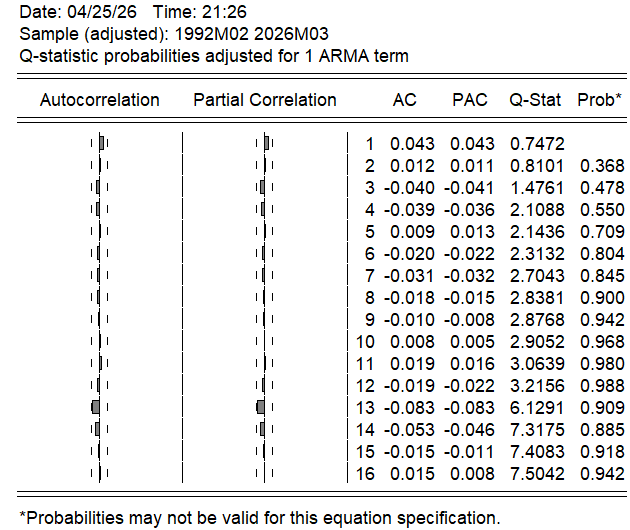
\includegraphics[width=0.7\textwidth]{序列DF_LN_WTI的MA(1)-EGARCH(1,1)模型残差的Q检验结果图.png}
\caption{MA(1)-EGARCH(1,1)-t模型残差序列的 Q 检验结果图}
\label{fig:序列DF_LN_WTI的MA(1)-EGARCH(1,1)模型残差的Q检验结果图}
\end{figure}

由图~\ref{fig:序列DF_LN_WTI的MA(1)-EGARCH(1,1)模型残差的Q检验结果图}可知，滞后1至16阶的自相关系数（AC）与偏自相关系数（PAC）均未超出95\%置信区间，且各阶Q统计量对应的伴随概率均大于0.05的显著性水平，无法拒绝残差序列为白噪声的原假设。这表明MA(1)-EGARCH(1,1)-t模型已充分提取了序列的均值与波动信息，残差序列不再存在显著的自相关性，模型设定合理。


\subsubsection{条件异方差检验}

对序列DF\_LN\_WTI的MA(1)-EGARCH(1,1)-t模型的残差序列分别做滞后4、5、6阶的ARCH效应检验，结果如图~\ref{fig:MA(1)-EGARCH(1,1)-t模型的ARCH效应检验结果图}所示。
\begin{figure}[H]
\centering
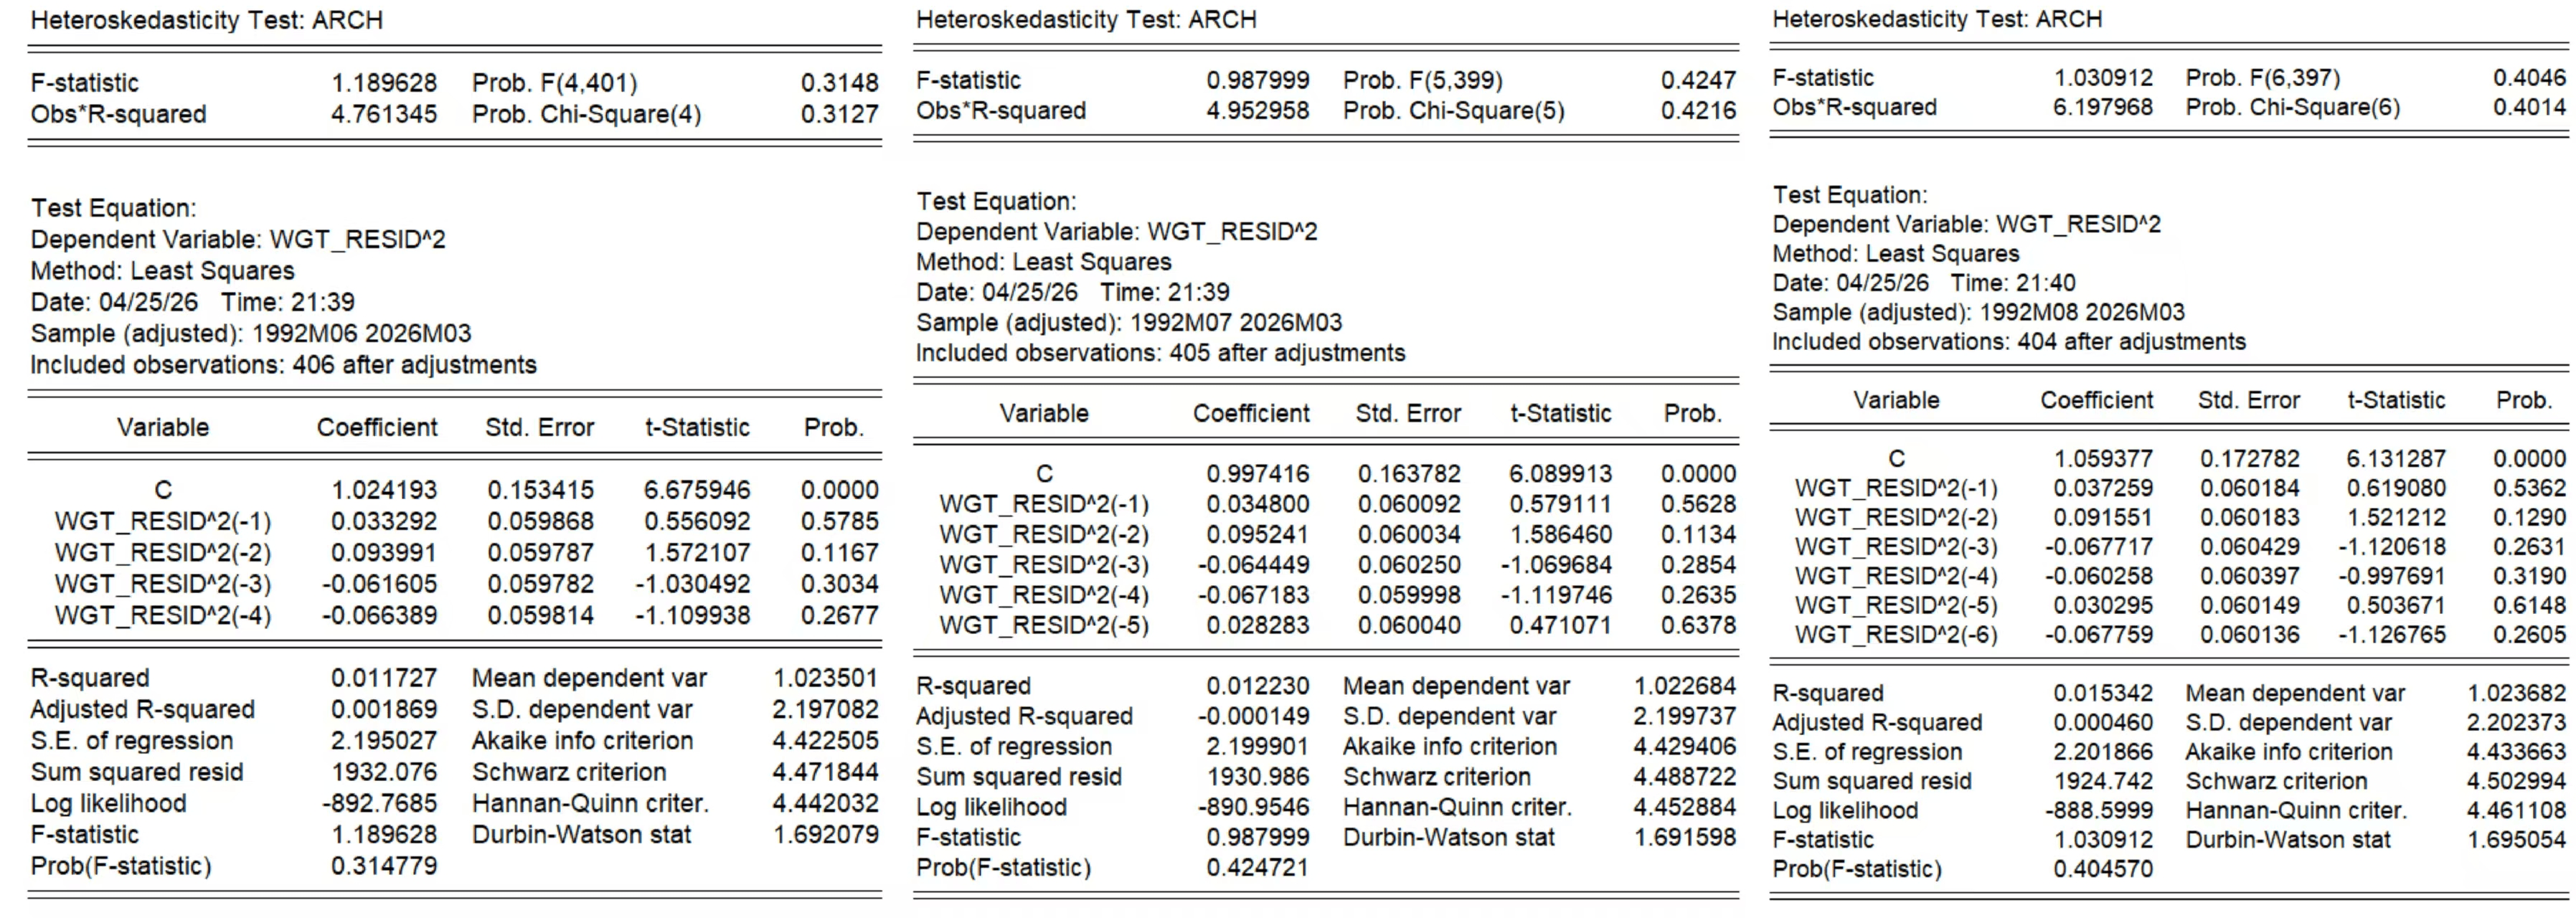
\includegraphics[width=0.8\textwidth]{MA(1)-EGARCH(1,1)-t模型的ARCH效应检验结果图.png}
\caption{MA(1)-EGARCH(1,1)-t模型的ARCH效应检验结果图}
\label{fig:MA(1)-EGARCH(1,1)-t模型的ARCH效应检验结果图}
\end{figure}

由图~\ref{fig:MA(1)-EGARCH(1,1)-t模型的ARCH效应检验结果图}可知，在滞后4、5、6阶条件下，ARCH-LM检验的伴随概率均远大于0.05的显著性水平，无法拒绝“残差不存在ARCH效应”的原假设。这表明MA(1)-EGARCH(1,1)-t模型已充分提取序列DF\_LN\_WTI的波动信息，残差序列不存在显著的条件异方差，模型设定合理且有效。



\subsection{模型方程与结果解读}

\subsubsection{模型方程与结果解读}

根据图~\ref{fig:egarch11}可知，序列DF\_LN\_WTI的MA(1)-EGARCH(1,1)-t模型的均值方程与方差方程形式如下：
\begin{align}\label{eq:序列DF_LN_WTI的MA(1)-EGARCH(1,1)-t模型均值方程}
\mathrm{DF}\_\mathrm{LN}\_\mathrm{WTI}_t=\varepsilon _t+\theta \varepsilon _{t-1}=\varepsilon _t+0.227205\cdot \varepsilon _{t-1},
\end{align}
\begin{gather}\label{eq:序列DF_LN_WTI的MA(1)-EGARCH(1,1)-t模型方差方程}
\begin{aligned}
\ln \left( \sigma _{t}^{2} \right) &=\omega +\alpha \left| \frac{\varepsilon _{t-1}}{\sigma _{t-1}} \right|+\gamma \frac{\varepsilon _{t-1}}{\sigma _{t-1}}+\beta \ln \left( \sigma _{t-1}^{2} \right) 
\\
&=-1.250255+0.297440\cdot \left| \frac{\varepsilon _{t-1}}{\sigma _{t-1}} \right|-0.162100\cdot \frac{\varepsilon _{t-1}}{\sigma _{t-1}}
\\
&\quad +0.797172\cdot \ln \left( \sigma _{t-1}^{2} \right) ,
\end{aligned}
\end{gather}
其中，$\varepsilon_t$ 为扰动项，$\sigma_t^2$ 为条件方差，$\theta$ 为移动平均系数，$\omega$ 为方差方程常数项，$\alpha$ 为ARCH项系数，$\gamma$ 为非对称项系数，$\beta$ 为GARCH项系数，模型扰动项$\varepsilon_t\sim t(9.407736)$。

均值方程\eqref{eq:序列DF_LN_WTI的MA(1)-EGARCH(1,1)-t模型均值方程}中，MA(1)系数$\theta=0.2272$在5\%水平下显著为正。其中$\mathrm{DF}\_\mathrm{LN}\_\mathrm{WTI}$为全球WTI原油现货价格的月度对数收益率，该结果表明WTI原油月度收益率存在显著的一阶移动平均特征，当期原油价格波动受前一期随机扰动的正向影响，原油价格波动具备短期记忆性特征。

由方差方程\eqref{eq:序列DF_LN_WTI的MA(1)-EGARCH(1,1)-t模型方差方程}可知
\begin{itemize}
\item ARCH项系数$\alpha=0.2974$显著为正，说明地缘政治冲突、原油供需格局变化、全球宏观经济波动等外部信息冲击，会显著加剧WTI原油现货价格的月度波动幅度。

\item GARCH项系数$\beta=0.7972$显著为正且接近1，体现出WTI原油价格波动具有极强的持续性，前期原油价格的大幅波动会持续传导至后续时期，符合国际原油市场波动聚集的典型特征。

\item 非对称项系数$\gamma=-0.1621$显著为负，证实WTI原油收益率序列存在显著\textbf{杠杆效应}，即原油需求下滑、地缘利空消息等负向冲击对价格波动的放大作用，显著强于供给收紧、经济利好等正向冲击。
\end{itemize}


\section{构建序列LN\_BRENT的时间序列模型}
\subsection{平稳性与非白噪声检验}
\subsubsection{ADF单位根检验}
对序列LN\_BRENT做ADF检验得到三种情形的p值分别为：None(0.8150)、Constant(0.4108)、Constant,Linear Trend(0.1999)均大于0.05，故原序列存在单位根，不满足平稳性。对其进行一阶差分得到序列
\begin{align}
\mathrm{DF}\_\mathrm{LN}\_\mathrm{BRENT}=\mathrm{LN}\_\mathrm{BRENT}_t-\mathrm{LN}\_\mathrm{BRENT}_{t-1},
\end{align}
再对差分后的序列重新进行ADF检验，检验结果如表~\ref{table:序列DF_LN_BRENT的ADF检验不同情形的信息准则对比}所示。
\begin{table}[H]
\centering
\caption{序列DF\_LN\_BRENT的ADF检验不同情形的信息准则对比}
\label{table:序列DF_LN_BRENT的ADF检验不同情形的信息准则对比}
\begin{tabular}{lcccc}
\toprule[1.2pt] % 顶部粗线
检验情形 & p值 &  AIC准则 & SC准则 & HQ准则 \\
\midrule[0.75pt] % 中间细线
None & 0.0000 & $\mathbf{-2.098702}$ & $\mathbf{-2.088888}$ & $\mathbf{-2.094819}$ \\
Constant & 0.0000 & -2.0953098 & -2.075682 & -2.087544 \\
Constant,Linear Trend & 0.0000 & -2.090420 & -2.060979 & -2.078771 \\
\bottomrule[1.2pt] % 底部粗线
\end{tabular}
\end{table}

由表~\ref{table:序列DF_LN_BRENT的ADF检验不同情形的信息准则对比}可知，三种检验情形下p值均小于0.05，拒绝存在单位根的原假设，序列平稳。根据AIC/SC/HQ信息准则，选择\textbf{无截距项、无时间趋势}的情形进行建模。


\subsubsection{自相关与偏自相关函数分析}

序列DF\_LN\_BRENT自相关与偏自相关函数检验结果如图~\ref{fig:序列DF_LN_BRENT的ACF和PACF相关图}所示。
\begin{figure}[H]
\centering
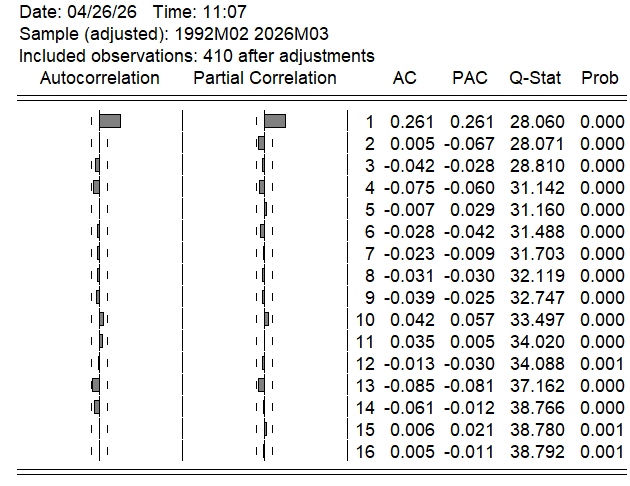
\includegraphics[width=0.8\textwidth]{序列DF_LN_BRENT的ACF和PACF相关图.png}
\caption{序列DF\_LN\_BRENT的ACF和PACF相关图}
\label{fig:序列DF_LN_BRENT的ACF和PACF相关图}
\end{figure}

由图~\ref{fig:序列DF_LN_BRENT的ACF和PACF相关图}可知，序列DF\_LN\_BRENT为非白噪声序列，其\textbf{自相关函数1阶截尾，偏自相关函数1阶截尾}。

\subsection{ARMA模型构建与条件异方差检验}
\subsubsection{模型构建与优选}

根据序列DF\_LN\_BRENT自相关与偏自相关函数的特征，对DF\_LN\_BRENT构建多种ARMA模型，并将各个ARMA模型的系数显著性检验结果和AIC/SC/HQ值汇总到如下表~\ref{tab:arma_pvalue_brent}中。
\begin{table}[H]
\centering
\caption{DF\_LN\_BRENT序列ARMA模型系数显著性检验和信息准则对比图}
\label{tab:arma_pvalue_brent}
\begin{tabular}{ccccccccc}
\toprule[1.2pt]
模型  & AR(1) & AR(2) & MA(1) & MA(2) & AIC & SC & HQ \\
\midrule[0.75pt]
ARMA(1,1)  & 0.6565 & - & 0.1044 & - & -2.0954 & -2.0660 & -2.0837 \\
ARMA(2,2)  & 0.0000 & 0.2551 & 0.0000 & 0.3959 & -2.0928 & -2.0438 & -2.0734 \\
ARMA(2,1)  & 0.0000 & 0.0000 & 0.0000 & -  & -2.0963 & -2.0571 & -2.0808 \\
ARMA(1,2)  & 0.9917 & - & 0.9190 & 0.9894 & -2.0905 & -2.0513 & -2.0750 \\
AR(1)      & 0.0000 & - & - & - & -2.0961 & -2.0765 & -2.0883 \\
AR(2)      & 0.0000 & 0.0953 & - & - & -2.0959 & -2.0665 & -2.0843 \\
MA(1)      & - & - & 0.0000 & - & $\mathbf{-2.1000}$ & $\mathbf{-2.0804}$ & $\mathbf{-2.0922}$ \\
MA(2)      & - & - & 0.0000 & 0.6528 & -2.0954 & -2.0660 & -2.0837 \\
\bottomrule[1.2pt]
\end{tabular}
\end{table}

由表~\ref{tab:arma_pvalue_brent}，再结合系数显著性与信息准则，最优均值模型为$\mathbf{MA}(\mathbf{1})$，模型结果如图~\ref{fig:序列DF_LN_BRENT的MA(1)模型结果图}所示。

\begin{figure}[H]
\centering
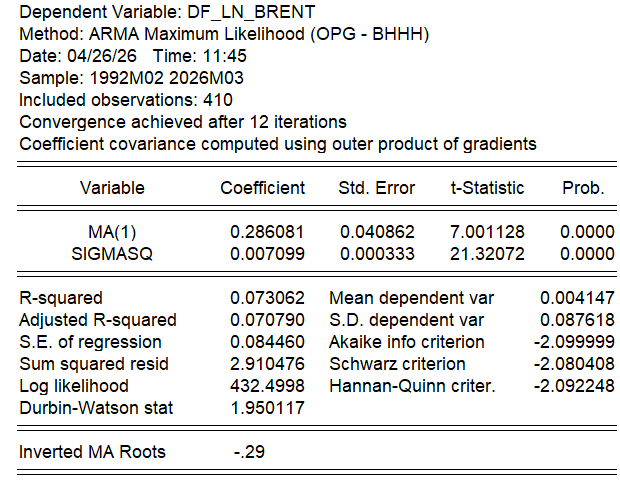
\includegraphics[width=0.8\textwidth]{序列DF_LN_BRENT的MA(1)模型结果图.png}
\caption{序列DF\_LN\_BRENT的MA(1)模型结果图}
\label{fig:序列DF_LN_BRENT的MA(1)模型结果图}
\end{figure}



\subsubsection{适应性与条件异方差检验}

序列DF\_LN\_BRENT的MA(1)模型的适应性检验结果如图~\ref{fig:序列DF_LN_BRENT的MA(1)模型适应性检验图}所示。

\begin{figure}[H]
\centering
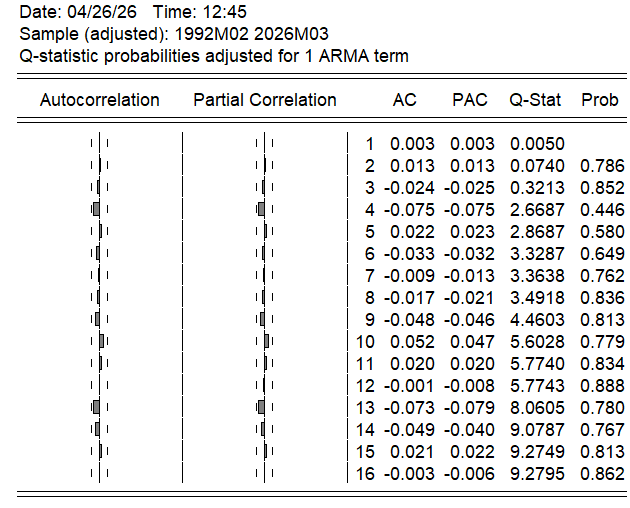
\includegraphics[width=0.8\textwidth]{序列DF_LN_BRENT的MA(1)模型适应性检验图.png}
\caption{序列DF\_LN\_BRENT的MA(1)模型适应性检验图}
\label{fig:序列DF_LN_BRENT的MA(1)模型适应性检验图}
\end{figure}

图~\ref{fig:序列DF_LN_BRENT的MA(1)模型适应性检验图}显示：MA(1)模型残差通过白噪声检验，均值信息提取充分。

序列DF\_LN\_BRENT的MA(1)模型的滞后4、5、6阶的ARCH-LM检验和残差平方序列的Q检验结果如图~\ref{fig:序列DF_LN_BRENT的MA(1)模型条件异方差检验图}所示。

\begin{figure}[H]
\centering
% 第一行
\begin{minipage}{0.48\textwidth}
\centering
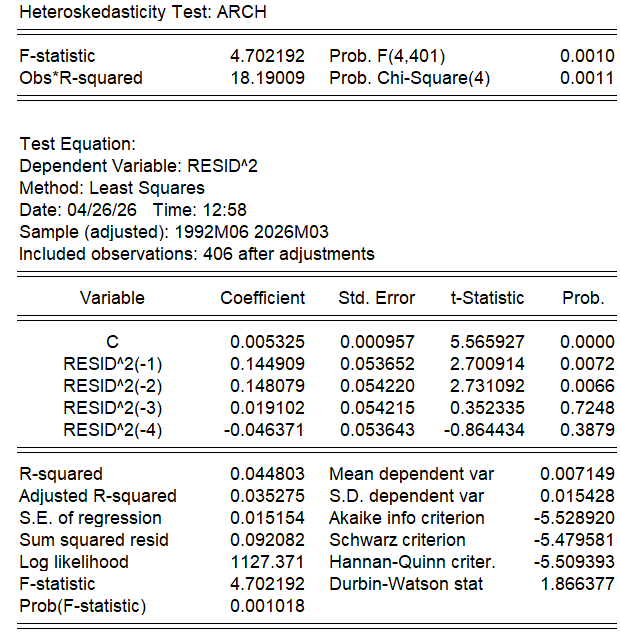
\includegraphics[width=\linewidth]{序列DF_LN_BRENT的MA(1)模型条件异方差检验图1.png}
\end{minipage}
\hfill
\begin{minipage}{0.48\textwidth}
\centering
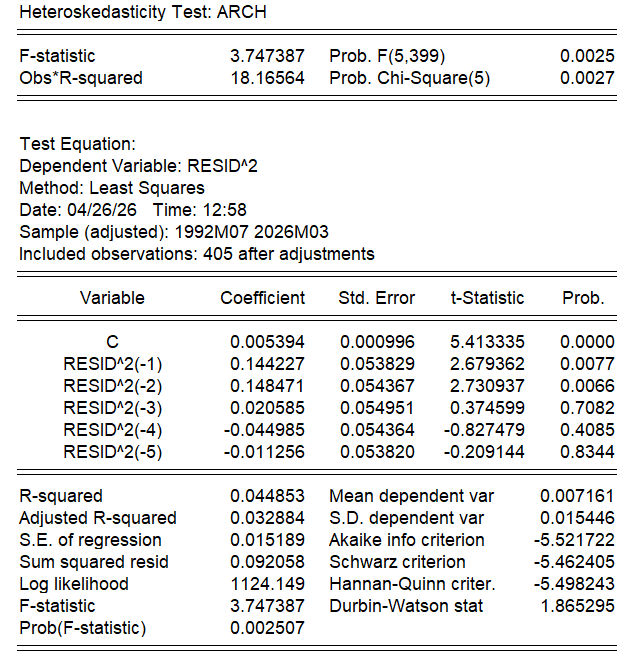
\includegraphics[width=\linewidth]{序列DF_LN_BRENT的MA(1)模型条件异方差检验图2.png}
\end{minipage}

\vspace{1em} % 上下行间距
% 第二行
\begin{minipage}{0.48\textwidth}
\centering
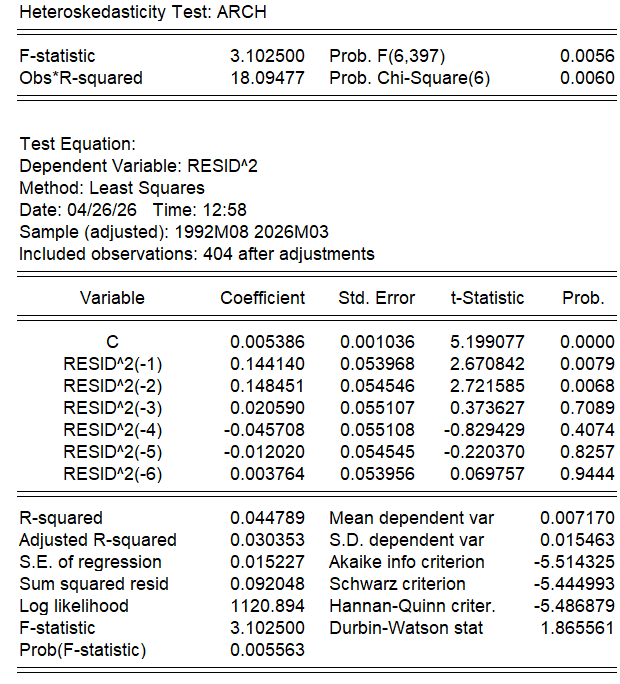
\includegraphics[width=\linewidth]{序列DF_LN_BRENT的MA(1)模型条件异方差检验图3.png}
\end{minipage}
\hfill
\begin{minipage}{0.48\textwidth}
\centering
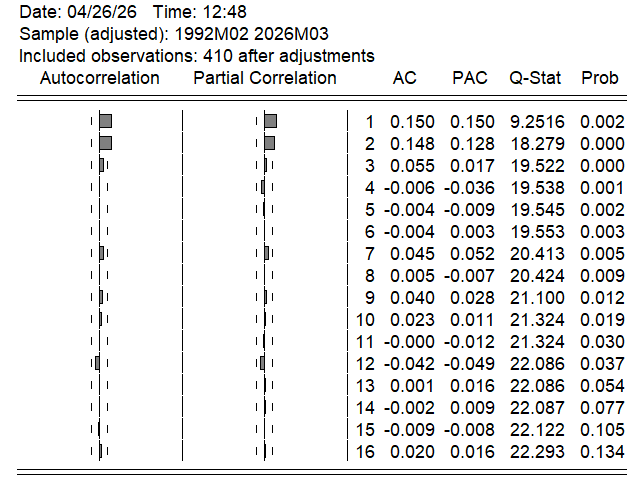
\includegraphics[width=\linewidth]{序列DF_LN_BRENT的MA(1)模型条件异方差检验图4.png}
\end{minipage}

\caption{序列DF\_LN\_BRENT的MA(1)模型条件异方差检验图}
\label{fig:序列DF_LN_BRENT的MA(1)模型条件异方差检验图}
\end{figure}

图~\ref{fig:序列DF_LN_BRENT的MA(1)模型条件异方差检验图}显示：残差序列存在显著的条件异方差性。为此，本文进一步构建GARCH族模型。

\subsection{GARCH族模型构建与检验}

序列DF\_LN\_BRENT的直方图与描述性统计如图~\ref{fig:序列DF_LN_BRENT的直方图与描述性统计图}所示。
\begin{figure}[H]
\centering
\includegraphics[width=0.8\textwidth]{序列DF\_LN\_BRENT的直方图与描述性统计图.png}
\caption{序列DF\_LN\_BRENT的直方图与描述性统计图}
\label{fig:序列DF_LN_BRENT的直方图与描述性统计图}
\end{figure}

由图~\ref{fig:序列DF_LN_BRENT的直方图与描述性统计图}可知，序列DF\_LN\_BRENT同样具备\textbf{尖峰厚尾}特征，故采用t分布构建GARCH族模型。将各GARCH族模型系数显著性检验和信息准则结果分别汇总到表~\ref{tab:garch_pvalue_brent1}和表~\ref{tab:garch_info_criteria_brent1}中。

\begin{table}[H]
\centering
\caption{DF\_LN\_BRENT序列GARCH族模型系数显著性检验结果}
\label{tab:garch_pvalue_brent1}
\setlength{\tabcolsep}{8pt}
\begin{tabular}{lcccc}
\toprule[1.2pt]
模型名称 & 常数项C & ARCH项 & 非对称项 & GARCH项 \\
\midrule[0.75pt]
MA(1)-GARCH(1,0)-t & \textbf{0.0000} & \textbf{0.0020} & - & - \\
MA(1)-GARCH(2,0)-t & 0.0000 & 0.0119 / 0.1624 & - & - \\
MA(1)-GARCH(1,1)-t & 0.0711 & 0.0106 & - & 0.0000 \\
MA(1)-GARCH(1,2)-t & 0.1173 & 0.0247 & - & 0.3410 / 0.6248 \\
MA(1)-GARCH(2,1)-t & 0.2584 & 0.0091 / 0.1120 & - & 0.0000 \\
MA(1)-GARCH(2,2)-t & 0.4571 & 0.0124 / 0.0557 & - & 0.0162 / 0.6028 \\
\midrule
MA(1)-TARCH(1,0)-t & 0.0000 & 0.4087 & 0.0027 & - \\
MA(1)-TARCH(2,0)-t & 0.0000 & 0.5153 / 0.3085 & 0.0049 & - \\
MA(1)-TARCH(1,1)-t & 0.0000 & 0.6256 & 0.0044 & 0.4610 \\
MA(1)-TARCH(1,2)-t & 0.0160 & 0.5665 & 0.0077 & 0.8394 / 0.0148 \\
MA(1)-TARCH(2,1)-t & 0.0001 & 0.6992 / 0.3794 & 0.0056 & 0.7249 \\
MA(1)-TARCH(2,2)-t & 0.0060 & 0.5901 / 0.3148 & 0.0031 & 0.5210 / 0.3916 \\
\midrule
MA(1)-EGARCH(1,0)-t & \textbf{0.0000} & \textbf{0.0094} & \textbf{0.0081} & - \\
MA(1)-EGARCH(2,0)-t & \textbf{0.0000} & \textbf{0.0164} / \textbf{0.0096} & \textbf{0.0168} & - \\
MA(1)-EGARCH(1,1)-t & 0.0310 & 0.0130 & 0.1428 & 0.0000 \\
MA(1)-EGARCH(1,2)-t & 0.0627 & 0.0067 & 0.0121 & 0.2432 / 0.0000 \\
MA(1)-EGARCH(2,1)-t & 0.0681 & 0.0246 / 0.6542 & 0.1683 & 0.0000 \\
MA(1)-EGARCH(2,2)-t & 0.0365 & 0.0107 / 0.1686 & 0.0384 & 0.7327 / 0.0000 \\
\bottomrule[1.2pt]
\end{tabular}
\end{table}

\begin{table}[H]
\centering
\caption{DF\_LN\_BRENT序列GARCH族模型信息准则结果对比}
\label{tab:garch_info_criteria_brent1}
\setlength{\tabcolsep}{12pt}
\begin{tabular}{lcccc}
\toprule[1.2pt]
模型名称 & MA(1)系数 & AIC & SC & HQ \\
\midrule[0.75pt]
MA(1)-GARCH(1,0)-t & 0.187003 & -2.2038 & -2.1646 & -2.1883 \\
MA(1)-GARCH(2,0)-t & 0.217883 & -2.2071 & -2.1581 & -2.1877 \\
MA(1)-GARCH(1,1)-t & 0.227823 & -2.2190 & -2.1700 & -2.1996 \\
MA(1)-GARCH(1,2)-t & 0.223801 & -2.2153 & -2.1566 & -2.1921 \\
MA(1)-GARCH(2,1)-t & 0.213462 & -2.2204 & -2.1616 & -2.1971 \\
MA(1)-GARCH(2,2)-t & 0.218747 & -2.2171 & -2.1485 & -2.1900 \\
\midrule
MA(1)-TARCH(1,0)-t & 0.230716 & -2.2274 & -2.1784 & -2.2080 \\
MA(1)-TARCH(2,0)-t & 0.237428 & -2.2263 & -2.1676 & -2.2031 \\
MA(1)-TARCH(1,1)-t & 0.236274 & -2.2236 & -2.1648 & -2.2003 \\
MA(1)-TARCH(1,2)-t & 0.220951 & -2.2232 & -2.1546 & -2.1961 \\
MA(1)-TARCH(2,1)-t & 0.237013 & -2.2216 & -2.1530 & -2.1945 \\
MA(1)-TARCH(2,2)-t & 0.229717 & -2.2236 & -2.1452 & -2.1926 \\
\midrule
MA(1)-EGARCH(1,0)-t & 0.235877 & -2.2009 & -2.1520 & -2.1816 \\
MA(1)-EGARCH(2,0)-t & \textbf{0.243346} & \textbf{-2.2174} & \textbf{-2.1587} & \textbf{-2.1942} \\
MA(1)-EGARCH(1,1)-t & 0.233722 & -2.2256 & -2.1668 & -2.2024 \\
MA(1)-EGARCH(1,2)-t & 0.226163 & -2.2277 & -2.1591 & -2.2005 \\
MA(1)-EGARCH(2,1)-t & 0.229811 & -2.2212 & -2.1526 & -2.1941 \\
MA(1)-EGARCH(2,2)-t & 0.234614 & -2.2297 & -2.1513 & -2.1987 \\
\bottomrule[1.2pt]
\end{tabular}
\end{table}

由表~\ref{tab:garch_pvalue_brent1}和表~\ref{tab:garch_info_criteria_brent1}，再结合显著性检验和信息准则可知，$\mathbf{MA}\left( \mathbf{1} \right) -\mathbf{EGARCH}\left( \mathbf{2},\mathbf{0} \right) -\mathbf{t}$为最优模型，所有参数均显著且信息准则表现最优，其结果如图~\ref{fig:序列DF_LN_BRENT的MA(1)-EGARCH(2,0)-t模型结果图}所示。

\begin{figure}[H]
\centering
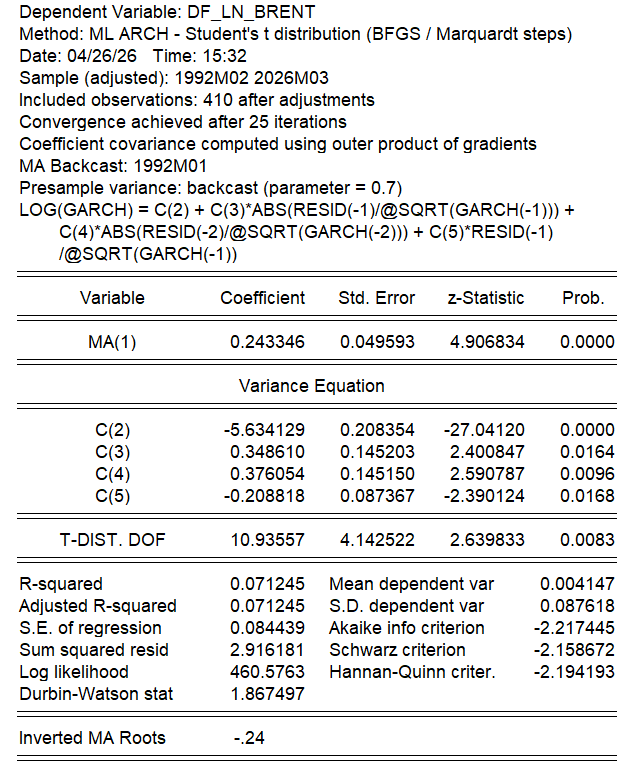
\includegraphics[width=0.8\textwidth]{序列DF_LN_BRENT的MA(1)-EGARCH(2,0)-t模型结果图.png}
\caption{MA(1)-EGARCH(2,0)-t模型结果图}
\label{fig:序列DF_LN_BRENT的MA(1)-EGARCH(2,0)-t模型结果图}
\end{figure}

MA(1)-EGARCH(2,0)-t模型的ARCH-LM检验(滞后4、5、6阶)和残差平方序列的Q检验结果如图~\ref{fig:MA(1)-EGARCH(2,0)-t模型的条件异方差检验结果图}所示。

\begin{figure}[H]
\centering
% 第一行
\begin{minipage}{0.48\textwidth}
\centering
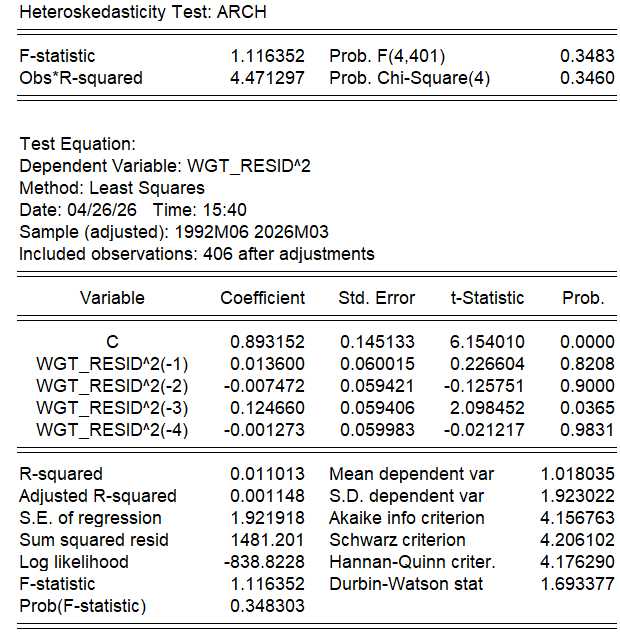
\includegraphics[width=\linewidth]{A(1)-EGARCH(2,0)-t模型的条件异方差检验结果图1.png}
\end{minipage}
\hfill
\begin{minipage}{0.48\textwidth}
\centering
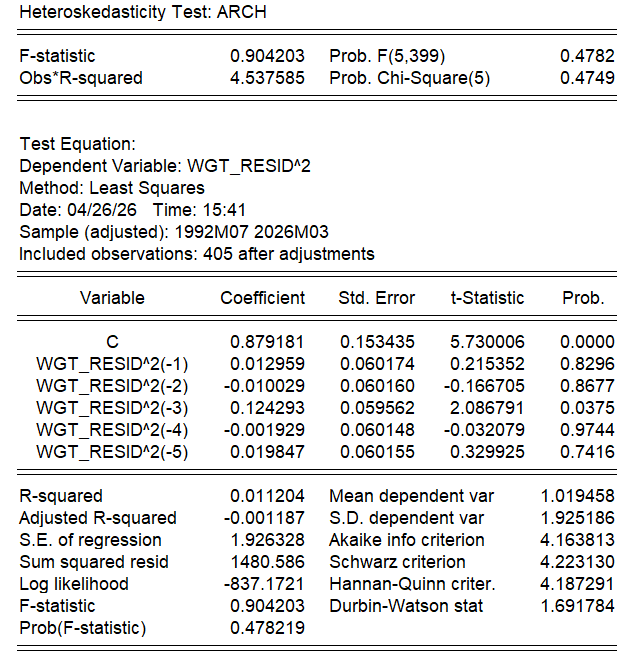
\includegraphics[width=\linewidth]{A(1)-EGARCH(2,0)-t模型的条件异方差检验结果图2.png}
\end{minipage}

\vspace{1em} % 上下行间距
% 第二行
\begin{minipage}{0.48\textwidth}
\centering
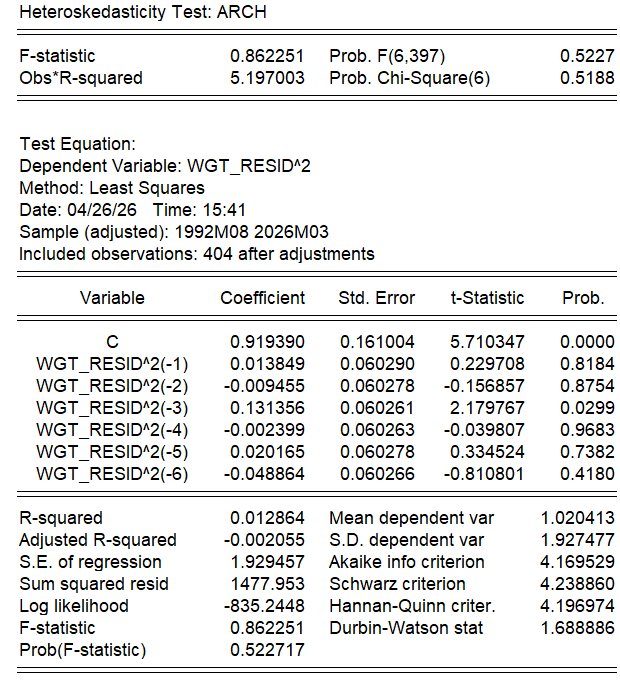
\includegraphics[width=\linewidth]{A(1)-EGARCH(2,0)-t模型的条件异方差检验结果图3.png}
\end{minipage}
\hfill
\begin{minipage}{0.48\textwidth}
\centering
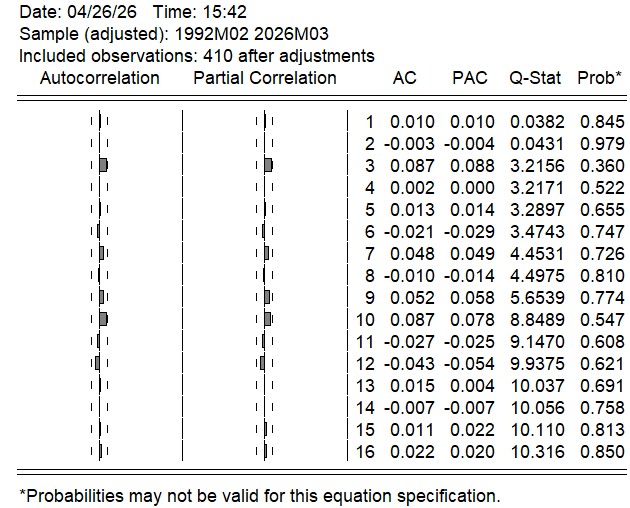
\includegraphics[width=\linewidth]{a(1)-egarch(2,0)-t模型的条件异方差检验结果图4.png}
\end{minipage}

\caption{MMA(1)-EGARCH(2,0)-t模型的条件异方差检验结果图}
\label{fig:MA(1)-EGARCH(2,0)-t模型的条件异方差检验结果图}
\end{figure}

根据图~\ref{fig:MA(1)-EGARCH(2,0)-t模型的条件异方差检验结果图}可知，各滞后期的p值均大于0.05，表明残差序列不存在显著自相关。结合ARCH-LM检验结果可知，滞后4、5、6阶的p值均大于0.05，这说明模型已充分捕捉原序列的条件异方差。

MA(1)-EGARCH(2,0)-t模型的残差白噪声检验结果如图~\ref{fig:MA(1)-EGARCH(2,0)-t模型的残差白噪声检验结果图}所示。

\begin{figure}[H]
\centering
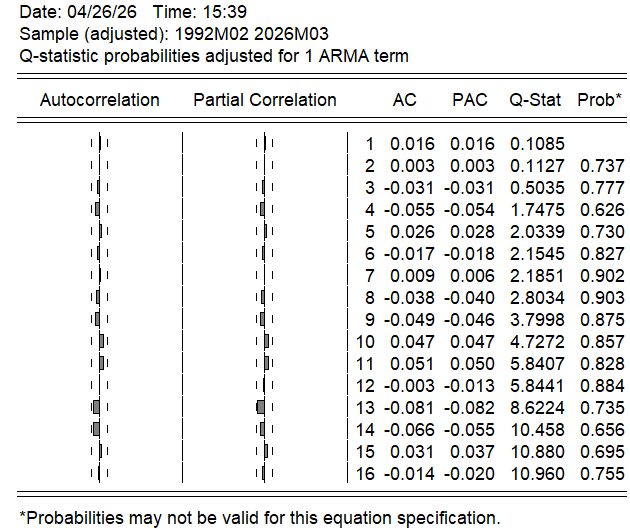
\includegraphics[width=0.8\textwidth]{MA(1)-EGARCH(2,0)-t模型的残差白噪声检验结果图.png}
\caption{MA(1)-EGARCH(2,0)-t模型的残差白噪声检验结果图}
\label{fig:MA(1)-EGARCH(2,0)-t模型的残差白噪声检验结果图}
\end{figure}

根据图~\ref{fig:MA(1)-EGARCH(2,0)-t模型的残差白噪声检验结果图}可知，各滞后阶数的p值均大于0.05，不拒绝残差序列为白噪声的原假设，表明模型已充分提取时间序列的动态信息。


\subsection{模型方程与结果解读}

由图~\ref{fig:序列DF_LN_BRENT的MA(1)-EGARCH(2,0)-t模型结果图}可知，序列DF\_LN\_BRENT的MA(1)-EGARCH(2,0)-t模型方程如下：
\begin{align}\label{eq:序列DF_LN_BRENT的MA(1)-EGARCH(2,0)-t模型均值方程}
\mathrm{DF}\_\mathrm{LN}\_\mathrm{BRENT}_t=\varepsilon _t+\theta \varepsilon _{t-1}=\varepsilon _t+0.243346\cdot \varepsilon _{t-1},
\end{align}
\begin{gather}\label{eq:序列DF_LN_BRENT的MA(1)-EGARCH(2,0)-t模型方差方程}
\begin{aligned}
\ln \left( \sigma _{t}^{2} \right) &=\omega +\alpha \left| \frac{\varepsilon _{t-1}}{\sigma _{t-1}} \right|+\gamma \frac{\varepsilon _{t-1}}{\sigma _{t-1}}+\beta \ln \left( \sigma _{t-1}^{2} \right) 
\\
&=-5.634129+0.348610\cdot \left| \frac{\varepsilon _{t-1}}{\sigma _{t-1}} \right|0.376054\cdot \frac{\varepsilon _{t-1}}{\sigma _{t-1}}
\\
&\quad -0.208818\cdot \ln \left( \sigma _{t-1}^{2} \right) ,
\end{aligned}
\end{gather}
其中，$\varepsilon_t$ 为扰动项，$\sigma_t^2$ 为条件方差，$\theta$ 为移动平均系数，$\omega$ 为方差方程常数项，$\alpha$ 为ARCH项系数，$\gamma$ 为非对称项系数，$\beta$ 为GARCH项系数，模型扰动项$\varepsilon_t\sim t(10.9.557)$。

上述均值方程\eqref{eq:序列DF_LN_BRENT的MA(1)-EGARCH(2,0)-t模型方差方程}和方差方程\eqref{eq:序列DF_LN_BRENT的MA(1)-EGARCH(2,0)-t模型方差方程}表明：\textbf{布伦特原油收益率存在短期记忆性，外部冲击会加剧价格波动，波动具有强持续性，且存在显著的负向杠杆效应。}

\newpage



\section{构建序列LN\_DUBAI的时间序列模型}

\subsection{平稳性与非白噪声检验}

\subsubsection{ADF单位根检验}

对序列LN\_DUBAI做ADF检验得到三种情形的p值分别为：None(0.8489)、Constant(0.4904)、Constant,Linear Trend(0.1390)均大于0.05，故原序列存在单位根，不满足平稳性。对其进行一阶差分得到序列
\begin{align}
\mathrm{DF}\_\mathrm{LN}\_\mathrm{DUBAI}=\mathrm{LN}\_\mathrm{DUBAI}_t-\mathrm{LN}\_\mathrm{DUBAI}_{t-1},
\end{align}
再对差分后的序列重新进行ADF检验，检验结果如表~\ref{table:序列DF_LN_DUBAI的ADF检验不同情形的信息准则对比}所示。

\begin{table}[H]
\centering
\caption{序列DF\_LN\_DUBAI的ADF检验不同情形的信息准则对比}
\label{table:序列DF_LN_DUBAI的ADF检验不同情形的信息准则对比}
\begin{tabular}{lcccc}
\toprule[1.2pt]
检验情形 & p值 & AIC准则 & SC准则 & HQ准则 \\
\midrule[0.75pt]
None & 0.0000 & \textbf{-2.076381} & \textbf{-2.066567} & \textbf{-2.072498} \\
Constant & 0.0000 & -2.073570 & -2.053943 & -2.065804 \\
Constant,Linear Trend & 0.0000 & -2.068842 & -2.039402 & -2.057194 \\
\bottomrule[1.2pt]
\end{tabular}
\end{table}

由表可知，三种检验情形下p值均小于0.05，拒绝存在单位根的原假设，序列平稳。根据AIC/SC/HQ信息准则，选择\textbf{无截距项、无时间趋势}的情形进行建模。


\subsubsection{自相关与偏自相关函数分析}

序列DF\_LN\_DUBAI自相关与偏自相关函数检验结果如图~\ref{fig:序列DF_LN_DUBAI的ACF和PACF相关图}所示。

\begin{figure}[H]
\centering
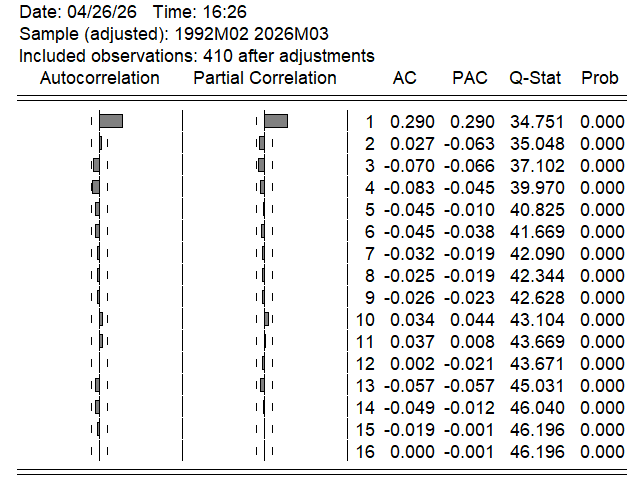
\includegraphics[width=0.8\textwidth]{序列DF_LN_DUBAI的ACF和PACF相关图.png}
\caption{序列DF\_LN\_DUBAI的ACF和PACF相关图}
\label{fig:序列DF_LN_DUBAI的ACF和PACF相关图}
\end{figure}

由图可知，序列DF\_LN\_DUBAI为非白噪声序列，其\textbf{自相关函数1阶截尾，偏自相关函数1阶截尾}。

\subsection{ARMA模型构建与条件异方差检验}

\subsubsection{模型构建与优选}

根据序列DF\_LN\_DUBAI自相关与偏自相关函数的特征，对DF\_LN\_DUBAI构建多种ARMA模型，并将各个ARMA模型的系数显著性检验结果和AIC/SC/HQ值汇总到如下表~\ref{tab:arma_pvalue_dubai}中。

\begin{table}[H]
\centering
\caption{DF\_LN\_DUBAI序列ARMA模型系数显著性检验和信息准则对比图}
\label{tab:arma_pvalue_dubai}
\begin{tabular}{ccccccccc}
\toprule[1.2pt]
模型 & AR(1) & AR(2) & MA(1) & MA(2) & AIC & SC & HQ \\
\midrule[0.75pt]
ARMA(1,1) & 0.1009 & - & 0.1818 & - & -2.072224 & -2.042838 & -2.060598 \\
ARMA(2,2) & 0.0000 & 0.0388 & 0.0000 & 0.6405 & -2.072927 & -2.023950 & -2.053551 \\
ARMA(2,1) & \textbf{0.0000} & \textbf{0.0000} & \textbf{0.0000} & - & -2.077152 & -2.037970 & -2.061651 \\
ARMA(1,2) & 0.8909 & - & 0.5020 & 0.6261 & -2.068641 & -2.029459 & -2.053139 \\
AR(1) & \textbf{0.0000} & - & - & - & -2.073362 & -2.053771 & -2.065611 \\
AR(2) & 0.0000 & 0.0769 & - & - & -2.073740 & -2.044354 & -2.062114 \\
MA(1) & - & - & \textbf{0.0000} & - & -2.073296 & -2.053705 & -2.065545 \\
MA(2) & - & - & \textbf{0.0000} & \textbf{0.0418} & -2.073392 & -2.044005 & -2.061765 \\
\bottomrule[1.2pt]
\end{tabular}
\end{table}

由表，再结合系数显著性与信息准则，最优均值模型为$\mathbf{AR}(\mathbf{1})$，模型结果如图~\ref{fig:序列DF_LN_DUBAI的AR(1)模型结果图}所示。

\begin{figure}[H]
\centering
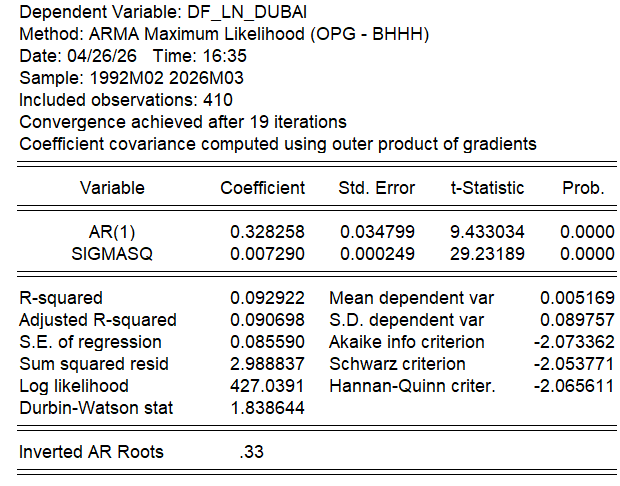
\includegraphics[width=0.8\textwidth]{序列DF_LN_DUBAI的AR(1)模型结果图.png}
\caption{序列DF\_LN\_DUBAI的AR(1)模型结果图}
\label{fig:序列DF_LN_DUBAI的AR(1)模型结果图}
\end{figure}

\subsubsection{适应性与条件异方差检验}

序列DF\_LN\_DUBAI的AR(1)模型的适应性检验结果如图~\ref{fig:序列DF_LN_DUBAI的AR(1)模型适应性检验图}所示。

\begin{figure}[H]
\centering
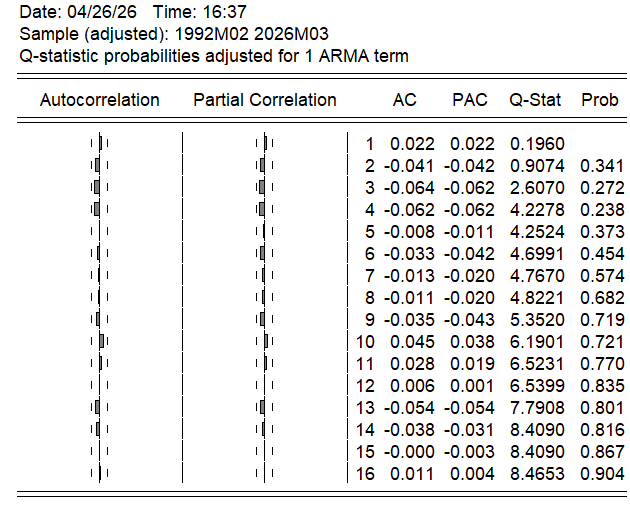
\includegraphics[width=0.8\textwidth]{序列DF_LN_DUBAI的AR(1)模型适应性检验图.png}
\caption{序列DF\_LN\_DUBAI的AR(1)模型适应性检验图}
\label{fig:序列DF_LN_DUBAI的AR(1)模型适应性检验图}
\end{figure}

图~\ref{fig:序列DF_LN_DUBAI的AR(1)模型适应性检验图}显示：AR(1)模型残差通过白噪声检验，均值信息提取充分。

序列DF\_LN\_DUBAI的AR(1)模型的滞后4、5、6阶的ARCH-LM检验和残差平方序列的Q检验结果如图~\ref{fig:序列DF_LN_DUBAI的AR(1)模型条件异方差检验图}所示。

\begin{figure}[H]
\centering
% 第一行
\begin{minipage}{0.48\textwidth}
\centering
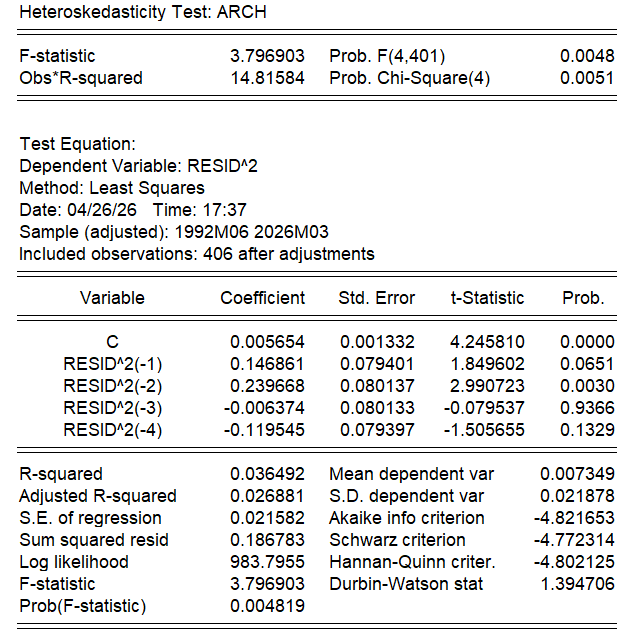
\includegraphics[width=\linewidth]{序列DF_LN_DUBAI的AR(1)模型条件异方差检验图1.png}
\end{minipage}
\hfill
\begin{minipage}{0.48\textwidth}
\centering
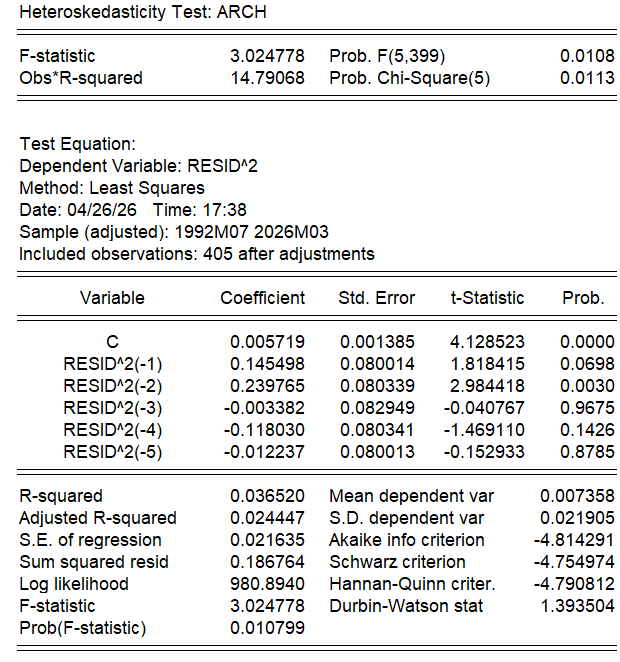
\includegraphics[width=\linewidth]{序列DF_LN_DUBAI的AR(1)模型条件异方差检验图2.png}
\end{minipage}

\vspace{1em}
% 第二行
\begin{minipage}{0.48\textwidth}
\centering
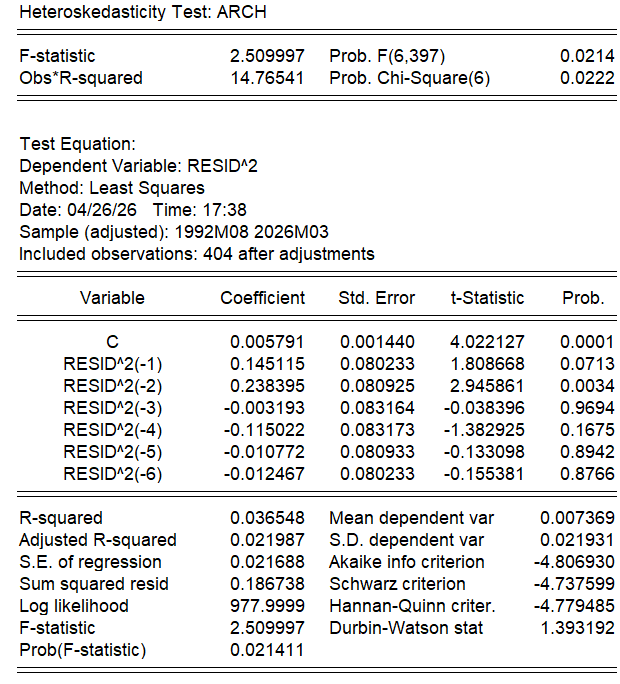
\includegraphics[width=\linewidth]{序列DF_LN_DUBAI的AR(1)模型条件异方差检验图3.png}
\end{minipage}
\hfill
\begin{minipage}{0.48\textwidth}
\centering
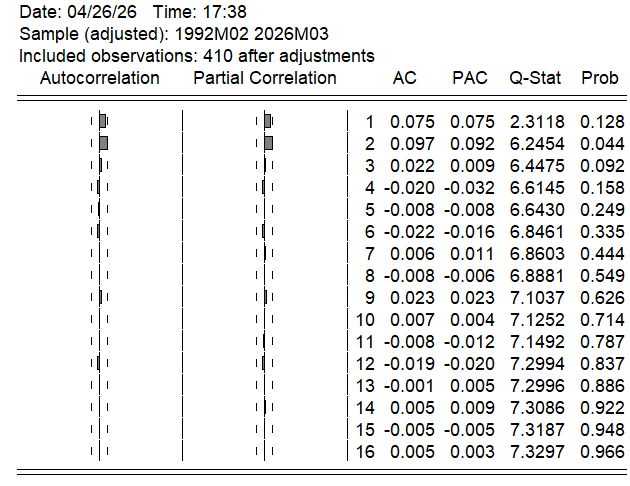
\includegraphics[width=\linewidth]{序列DF_LN_DUBAI的AR(1)模型条件异方差检验图4.png}
\end{minipage}

\caption{序列DF\_LN\_DUBAI的AR(1)模型条件异方差检验图}
\label{fig:序列DF_LN_DUBAI的AR(1)模型条件异方差检验图}
\end{figure}

图~\ref{fig:序列DF_LN_DUBAI的AR(1)模型条件异方差检验图}显示：残差序列存在显著的条件异方差性。为此，本文进一步构建GARCH族模型。

\subsection{GARCH族模型构建与检验}

序列DF\_LN\_DUBAI的直方图与描述性统计如图~\ref{fig:序列DF_LN_DUBAI的直方图与描述性统计图}所示。

\begin{figure}[H]
\centering
\includegraphics[width=0.8\textwidth]{序列DF_LN_DUBAI的直方图与描述性统计图.png}
\caption{序列DF\_LN\_DUBAI的直方图与描述性统计图}
\label{fig:序列DF_LN_DUBAI的直方图与描述性统计图}
\end{figure}

由图可知，序列DF\_LN\_DUBAI同样具备\textbf{尖峰厚尾}特征，故采用t分布构建GARCH族模型。将各GARCH族模型系数显著性检验和信息准则结果分别汇总到表~\ref{tab:garch_pvalue_dubai}和表~\ref{tab:garch_info_criteria_dubai}中。

\begin{table}[H]
\centering
\caption{DF\_LN\_DUBAI序列GARCH族模型系数显著性检验结果}
\label{tab:garch_pvalue_dubai}
\setlength{\tabcolsep}{8pt}
\begin{tabular}{lcccc}
\toprule[1.2pt]
模型名称 & 常数项C & ARCH项 & 非对称项 & GARCH项 \\
\midrule[0.75pt]
AR(1)-GARCH(1,0)-t     & 0.0000 & 0.0876 & - & - \\
AR(1)-GARCH(2,0)-t     & 0.0000 & 0.2283 / 0.2437 & - & - \\
AR(1)-GARCH(1,1)-t     & 0.1577 & 0.3083 & - & 0.6335 \\
AR(1)-GARCH(1,2)-t     & 0.0444 & 0.1967 & - & 0.1310 / 0.1013 \\
AR(1)-GARCH(2,1)-t     & 0.6293 & 0.3454 / 0.9815 & - & 0.8787 \\
AR(1)-GARCH(2,2)-t     & 0.0009 & 0.1269 / 0.1441 & - & 0.9455 / 0.2267 \\
\midrule
AR(1)-TARCH(1,0)-t     & 0.0000 & 0.2956 & 0.0063 & - \\
AR(1)-TARCH(2,0)-t     & 0.0000 & 0.3888 / 0.5015 & 0.0076 & - \\
AR(1)-TARCH(1,1)-t     & 0.0000 & 0.5026 & 0.0068 & 0.5418 \\
AR(1)-TARCH(1,2)-t     & 0.0001 & 0.5900 & 0.0057 & 0.6664 / 0.7452 \\
AR(1)-TARCH(2,1)-t     & 0.0000 & 0.5036 / 0.9671 & 0.0072 & 0.6278 \\
AR(1)-TARCH(2,2)-t     & 0.0000 & 0.5998 / 0.0964 & 0.0065 & 0.2366 / 0.9086 \\
\midrule
AR(1)-EGARCH(1,0)-t    & \textbf{0.0000} & \textbf{0.0013} & \textbf{0.0101} & - \\
AR(1)-EGARCH(2,0)-t    & \textbf{0.0000} & \textbf{0.0015} / \textbf{0.0137} & \textbf{0.0166} & - \\
AR(1)-EGARCH(1,1)-t    & \textbf{0.0118} & \textbf{0.0099} & \textbf{0.0218} & \textbf{0.0000} \\
AR(1)-EGARCH(1,2)-t    & 0.0205 & 0.0101 & 0.0171 & 0.0610 / 0.1884 \\
AR(1)-EGARCH(2,1)-t    & 0.0338 & 0.0183 / 0.7554 & 0.0175 & 0.0003 \\
AR(1)-EGARCH(2,2)-t    & 0.0390 & 0.0131 / 0.4136 & 0.0146 & 0.4972 / 0.0789 \\
\bottomrule[1.2pt]
\end{tabular}
\end{table}

\begin{table}[H]
\centering
\caption{DF\_LN\_DUBAI序列GARCH族模型信息准则结果对比}
\label{tab:garch_info_criteria_dubai}
\setlength{\tabcolsep}{12pt}
\begin{tabular}{lcccc}
\toprule[1.2pt]
模型名称 & AR(1)系数(p值) & AIC & SC & HQ \\
\midrule[0.75pt]
AR(1)-GARCH(1,0)-t     & 0.0000 & -2.150568 & -2.111314 & -2.135037 \\
AR(1)-GARCH(2,0)-t     & 0.0001 & -2.127236 & -2.078168 & -2.107822 \\
AR(1)-GARCH(1,1)-t     & 0.0003 & -2.044434 & -1.995366 & -2.025020 \\
AR(1)-GARCH(1,2)-t     & 0.0000 & -2.085860 & -2.026979 & -2.062563 \\
AR(1)-GARCH(2,1)-t     & 0.0018 & -2.046218 & -1.987337 & -2.022921 \\
AR(1)-GARCH(2,2)-t     & 0.0000 & -2.193008 & -2.124314 & -2.165828 \\
\midrule
AR(1)-TARCH(1,0)-t     & 0.0000 & -2.310822 & -2.261755 & -2.291408 \\
AR(1)-TARCH(2,0)-t     & 0.0000 & -2.308010 & -2.249129 & -2.284713 \\
AR(1)-TARCH(1,1)-t     & 0.0000 & -2.308616 & -2.249735 & -2.285319 \\
AR(1)-TARCH(1,2)-t     & 0.0000 & -2.304437 & -2.235743 & -2.277257 \\
AR(1)-TARCH(2,1)-t     & 0.0000 & -2.303728 & -2.235034 & -2.276548 \\
AR(1)-TARCH(2,2)-t     & 0.0000 & -2.304617 & -2.226109 & -2.273554 \\
\midrule
AR(1)-EGARCH(1,0)-t    & 0.0000 & -2.273970 & -2.224903 & -2.254556 \\
AR(1)-EGARCH(2,0)-t    & 0.0000 & -2.284499 & -2.225618 & -2.261202 \\
AR(1)-EGARCH(1,1)-t    & 0.0000 & \textbf{-2.296263} & \textbf{-2.237382} & \textbf{-2.272965} \\
AR(1)-EGARCH(1,2)-t    & 0.0000 & -2.294569 & -2.225875 & -2.267389 \\
AR(1)-EGARCH(2,1)-t    & 0.0000 & -2.291505 & -2.222811 & -2.264325 \\
AR(1)-EGARCH(2,2)-t    & 0.0000 & -2.292254 & -2.213746 & -2.261191 \\
\bottomrule[1.2pt]
\end{tabular}
\end{table}

由表，再结合显著性检验和信息准则可知，$\mathbf{MA}(\mathbf{1})-\mathbf{EGARCH}(\mathbf{1},\mathbf{1})-\mathbf{t}$为最优模型，所有参数均显著且信息准则表现最优，其结果如图~\ref{fig:序列DF_LN_DUBAI的MA(1)-EGARCH(1,1)模型结果图}所示。

\begin{figure}[H]
\centering
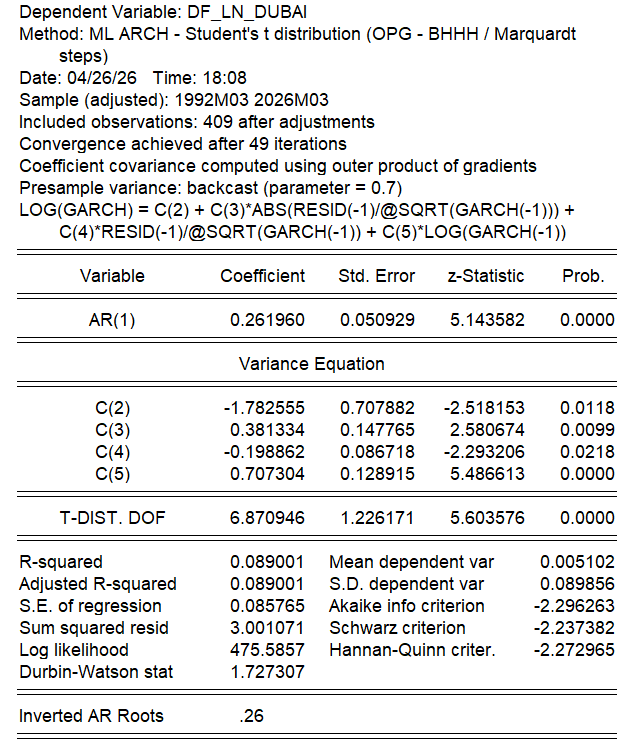
\includegraphics[width=0.8\textwidth]{序列DF_LN_DUBAI的MA(1)-EGARCH(1,1)模型结果图.png}
\caption{MA(1)-EGARCH(1,1)-t模型结果图}
\label{fig:序列DF_LN_DUBAI的MA(1)-EGARCH(1,1)模型结果图}
\end{figure}

MA(1)-EGARCH(1,1)-t模型的ARCH-LM检验（滞后4、5、6阶）和残差平方序列的Q检验结果如图~\ref{fig:MA(1)-EGARCH(1,1)-t模型的条件异方差检验结果图}所示。

\begin{figure}[H]
\centering
% 第一行
\begin{minipage}{0.48\textwidth}
\centering
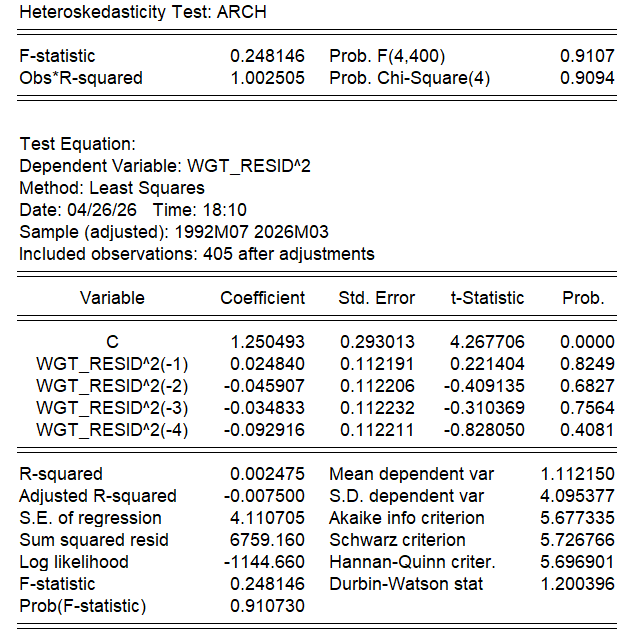
\includegraphics[width=\linewidth]{MA(1)-EGARCH(1,1)-t模型的条件异方差检验结果图1.png}
\end{minipage}
\hfill
\begin{minipage}{0.48\textwidth}
\centering
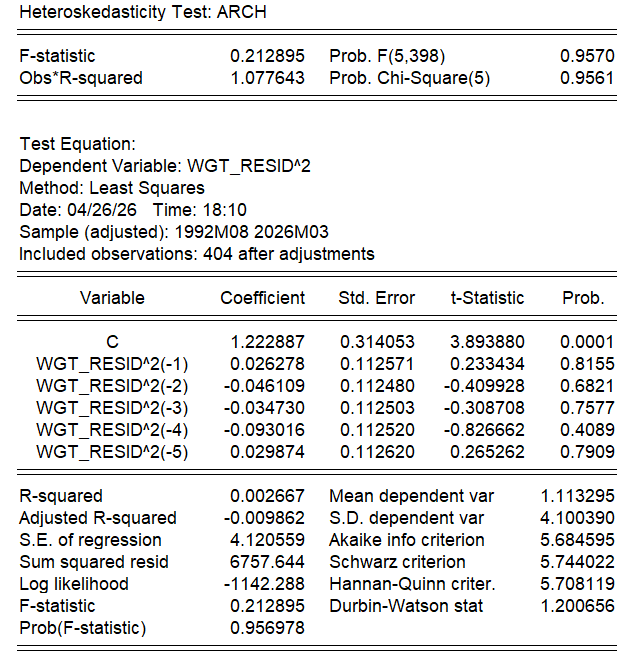
\includegraphics[width=\linewidth]{MA(1)-EGARCH(1,1)-t模型的条件异方差检验结果图2.png}
\end{minipage}

\vspace{1em}
% 第二行
\begin{minipage}{0.48\textwidth}
\centering
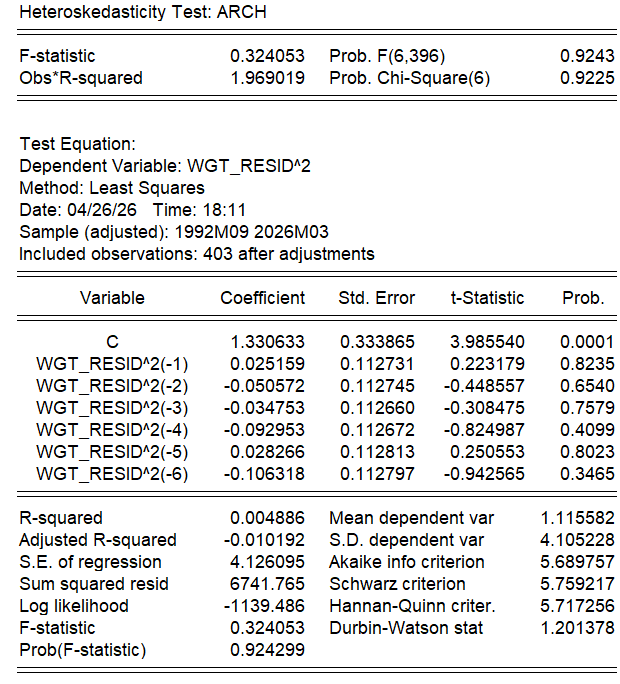
\includegraphics[width=\linewidth]{MA(1)-EGARCH(1,1)-t模型的条件异方差检验结果图3.png}
\end{minipage}
\hfill
\begin{minipage}{0.48\textwidth}
\centering
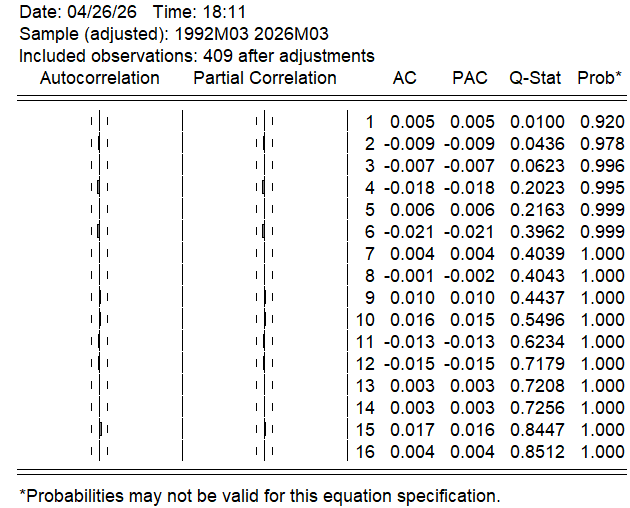
\includegraphics[width=\linewidth]{MA(1)-EGARCH(1,1)-t模型的条件异方差检验结果图4.png}
\end{minipage}

\caption{MA(1)-EGARCH(1,1)-t模型的条件异方差检验结果图}
\label{fig:MA(1)-EGARCH(1,1)-t模型的条件异方差检验结果图}
\end{figure}

根据图可知，各滞后期的p值均大于0.05，表明残差序列不存在显著自相关。结合ARCH-LM检验结果可知，滞后4、5、6阶的p值均大于0.05，这说明模型已充分捕捉原序列的条件异方差。

MA(1)-EGARCH(1,1)-t模型的残差白噪声检验结果如图~\ref{fig:MA(1)-EGARCH(1,1)-t模型的残差白噪声检验结果图}所示。

\begin{figure}[H]
\centering
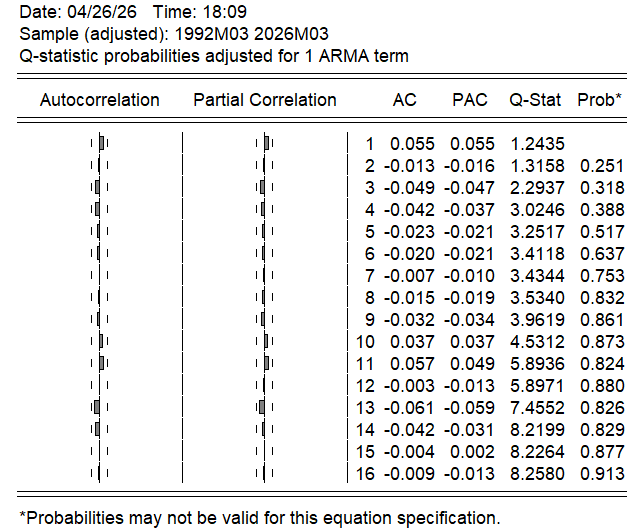
\includegraphics[width=0.8\textwidth]{MA(1)-EGARCH(1,1)-t模型的残差白噪声检验结果图.png}
\caption{MA(1)-EGARCH(1,1)-t模型的残差白噪声检验结果图}
\label{fig:MA(1)-EGARCH(1,1)-t模型的残差白噪声检验结果图}
\end{figure}

根据图可知，各滞后阶数的p值均大于0.05，不拒绝残差序列为白噪声的原假设，表明模型已充分提取时间序列的动态信息。

\subsection{模型方程与结果解读}

由图~\ref{fig:序列DF_LN_DUBAI的MA(1)-EGARCH(1,1)模型结果图}可知，序列DF\_LN\_DUBAI的MA(1)-EGARCH(1,1)-t模型方程如下：
\begin{align}\label{eq:序列DF_LN_DUBAI的MA(1)-EGARCH(1,1)-t模型均值方程}
\mathrm{DF}\_\mathrm{LN}\_\mathrm{DUBAI}_t=\varepsilon _t+\theta \varepsilon _{t-1}=\varepsilon _t+0.261960\cdot \varepsilon _{t-1},
\end{align}
\begin{gather}\label{eq:序列DF_LN_DUBAI的MA(1)-EGARCH(1,1)-t模型方差方程}
\begin{aligned}
\ln \left( \sigma _{t}^{2} \right) &=\omega +\alpha \left| \frac{\varepsilon _{t-1}}{\sigma _{t-1}} \right|+\gamma \frac{\varepsilon _{t-1}}{\sigma _{t-1}}+\beta \ln \left( \sigma _{t-1}^{2} \right) 
\\
&=-1.782555+ 0.381334\cdot \left| \frac{\varepsilon _{t-1}}{\sigma _{t-1}} \right|+-0.198862\cdot \frac{\varepsilon _{t-1}}{\sigma _{t-1}}
\\
&\quad + 0.707304\cdot \ln \left( \sigma _{t-1}^{2} \right) ,
\end{aligned}
\end{gather}
其中，$\varepsilon_t$ 为扰动项，$\sigma_t^2$ 为条件方差，$\theta$ 为移动平均系数，$\omega$ 为方差方程常数项，$\alpha$ 为ARCH项系数，$\gamma$ 为非对称项系数，$\beta$ 为GARCH项系数，模型扰动项$\varepsilon_t\sim t(6.870946)$。

上述均值方程和方差方程表明：\textbf{迪拜原油收益率存在短期记忆性，外部冲击会加剧价格波动，波动具有强持续性，且存在显著的负向杠杆效应。}



\section{三大原油价格波动特征对比分析}

\begin{itemize}
\item \textbf{波动共性}：三大国际原油价格均为一阶单整序列，最优均值模型均为MA(1)，最优波动模型均为MA(1)-EGARCH(1,1)-t；均存在短期记忆性、波动聚集性与负向杠杆效应，符合金融时间序列典型特征。
\item \textbf{区域差异}：Brent作为全球基准，杠杆效应最显著；WTI受北美市场影响，短期波动敏感性最强；Dubai作为亚太基准，波动持续性最强，体现了不同定价区域的市场结构差异。
\end{itemize}

\section{结论}

本文基于WTI、Brent和Dubai三大国际原油1992年1月至2026年3月的月度价格数据，采用ARMA-EGARCH模型系统分析了其对数收益率序列的波动特征。主要结论如下：

\begin{itemize}
\item 三大原油价格均为非平稳序列，一阶差分后平稳且为白噪声；最优均值模型分别为WTI和Brent为MA(1)，Dubai为AR(1)，表明原油市场具有短期可预测性。
\item 所有序列均存在显著的条件异方差和尖峰厚尾分布，t分布GARCH族模型能有效刻画波动聚集性。
\item 三大市场均存在显著的杠杆效应，负向冲击对价格波动的放大作用强于正向冲击，其中Brent的杠杆效应最强。
\item 波动持续性方面，WTI最高（$\beta=0.7972$），Brent无GARCH项，冲击衰减最快；Dubai的ARCH项最大，对即期信息反应最敏感。这些差异反映了三大区域市场结构、交易机制和定价权本质的不同。
\end{itemize}

本研究为国际原油市场的风险管理、衍生品定价及政策调控提供了量化依据，同时也验证了EGARCH-t模型在能源商品市场波动建模中的适用性。






% 参考文献
% \begin{thebibliography}{99}
% \bibitem{1} 王振山. 金融时间序列分析[M]. 北京: 北京大学出版社, 2020.
% \bibitem{2} 高铁梅. 计量经济分析方法与建模[M]. 北京: 清华大学出版社, 2019.
% \bibitem{3} 张晓峒. 时间序列分析[M]. 北京: 经济科学出版社, 2021.
% \end{thebibliography}












\end{document}